\chapter{Matrices}	

\section[Matrices: definición, tipo o dimensión e igualdad]{Matrices: definición, tipo o dimensión e igualdad} \sectionmark{Matrices. Definición}
\sectionmark{Matrices. Definición}

En adelante, $\mathbb K$ será uno de los cuerpos $\mathbb Q, \; \mathbb R, \; \mathbb C$;  $\; m$ y $n$ representarán números naturales:

\begin{defi} Una `matriz' es un tablero rectangular que contendrá elementos del cuerpo $\mathbb K$. La matriz será una colección de filas y columnas de números (aunque podían ser vectores, funciones, etc). 	
\end{defi}
\begin{defi}
Se llama `dimensión' o `tipo' de una matriz	al `número (indicado, no multiplicado)  de filas' por `número de columnas', así, una matriz de tipo $m\times n$, que representaremos por letras mayúsculas $A$, p.e., será un tablero rectangular que contendrá $m$-filas y $n$-columnas de números (que representaremos por letras minúsculas $a_{ij}$, haciendo referencia el primer índice $i$ a la fila que ocupa el elemento y el segundo índice $j$ a la columna en que está).

\begin{myblock}{Matriz $\boldsymbol{A_{m\; x \; n}}$}

$A=\left[
\begin{matrix}
a_{11} & a_{12} & \cdots & a_{1j} & \cdots & a_{1n} \\
a_{21} & a_{22} & \cdots & a_{2j} & \cdots & a_{2n} \\
a_{31} & a_{32} & \cdots & a_{3j} & \cdots & a_{3n} \\
\vdots & \vdots & \ddots & \vdots & \ddots & \vdots \\
a_{i1} & a_{i2} & \cdots & \boxed{a_{ij}} & \cdots & a_{in} \\
\vdots & \vdots & \ddots & \vdots & \ddots & \vdots \\
a_{m1} & a_{m2} & \cdots & a_{mj} & \cdots & a_{mn} \\
\end{matrix}
\right]$
\footnotesize{$= [a_{ij}]_{m \times n} \; \begin{cases}0\le i \le m; \\ 0\le j \le n\end{cases}$}

\vspace{3mm}
\centerline{$\boxed{\; \boldsymbol{A_{\;  (num. \; filas)\; \times \; (num. \; columnas) }}\; }$}

\end{myblock}

\end{defi}
 
Los elementos $a_{i1}, a_{i2}, \cdots , a_{in}$ forman la `fila i-ésima'

Los elementos $a_{1j}, a_{2j}, \cdots , a_{mj}$ forman la `columna j-ésima'

Por ejemplo: \hspace{2mm} fila-2 $\; (a_{21}, a_{22}, \cdots , a_{2n})\; $;\hspace{2mm} columna 3 $\; \left(\begin{matrix} a_{12} \\ a_{23}\\ \vdots \\ a_{m3}   \end{matrix}  \right)$. 

De este modo puede considerar a $A$ como una matriz de m-filas o de n-columnas:
$\quad A \quad=\quad \left( \begin{matrix} f_1 \\f_2\\ \vdots \\ f_m \end{matrix} \right) \quad = \quad  (\;c_1, c_2, \cdots, c_n \;)$


\begin{defi}Igualdad de matrices.

Dos matrices son iguales si, siendo del mismo tipo, tienen los mismos elementos en las misma posiciones:

$\quad { \left( { a }_{ ij } \right)  }_{ \begin{matrix} 1\le 1\le m \\ 1\le i\le n \end{matrix} }$
$\; = \; $
${ \left( { b }_{ ij } \right)  }_{ \begin{matrix} 1\le 1\le m \\ 1\le i\le n \end{matrix} } \leftrightarrow a_{ij}=b_{ij}; \; \forall i,j$

\end{defi}

En lo sucesivo llamaremos $\boldsymbol{ \mathcal M_{m\times n}(\mathbb K) }$ al conjunto de todas las matrices de tipo $m\times n$ sobre el cuerpo $\mathbb K$. Y, en general, mientras no se diga lo contrario, consideraremos $\mathbb K=\mathbb R$, hablaremos de matrices de números reales.

\subsection{Matriz traspuesta}

\begin{defi} Dada $A_{m\times n}\in \mathcal M_{m\times n}(\mathbb R)$, se llama `matriz traspuesta' de $A$ y se denota por $A^T$ a la matriz que resulta de `cambiar en $A$ las filas por las columnas' (o viceversa), es decir:

$A^T_{n\times m} = (A_{m\times n})^T\; :\;  \; $ si  $\quad$ \colorbox{LightYellow}{$\boxed{ \; A=(a_{ij}) \to A^T=(a_{ji})\; }$	}
\end{defi}

\begin{ejem}
$A_{2\times 3}=\left( \begin{matrix} 1 & 2 & 3 \\ 4 & 5 & 6 \end{matrix} \right)	 \to A^T_{3\times 2}= \left( \begin{matrix} 1 & 4 \\ 2 & 5 \\ 3 & 6 \end{matrix} \right)	 $

\noindent \small{$B_{4\times 1}=\left( \begin{matrix} 1 \\ 2 \\ 3 \\ 4 \end{matrix} \right) \to B^T_{1\times 4}= (\;1,2,3,4 \; ) \; ; \qquad C_{1\times 3}= (\;x,y,z \;) \to C^T_{3\times 1}=\left( \begin{matrix} x \\ y \\ z \end{matrix} \right)$}
\end{ejem}

\begin{prop}{Propiedad de la matriz traspuesta}
\label{propo1}

$A_{m\times n}\in \mathcal M_{m\times n}(\mathbb R) \to\; \boxed{\; \boldsymbol{ (A^T)^T=A}\; } $ 	
\end{prop}

\begin{proof}.

Evidentemente: $A=(a_{ij}) \to A^T=(a_{ji}) \Rightarrow (A^T)^T=(a_{ij})=A$	
\end{proof}


\section{Matrices especiales}

\begin{defi} `Matriz Cuadrada': son matrices del tipo $n\times n$, es decir, que tienen el `mismo número de filas que de columnas'.

Los elementos de la forma $a_{ii}$ se llaman `elementos diagonales' y a la línea en que están situados se le llama `diagonal principal'.
\end{defi}
\begin{defi}
`Matriz Diagonal' es una matriz cuadrada en la que los elementos que no están en la diagonal principal valen todos cero: $a_{ij}=0, \; \forall i \neq j$	
\end{defi}
\begin{defi} `Matriz Identidad o Unidad', es una matriz diagonal con los elementos de la diagonal ppal. iguales a uno. $a_{ii}=1; \; a_{ij}=0, \; \forall i \neq j$	
\end{defi}
 A las matrices cuadradas del tipo $A_{n \times n}$ se les suele llamar matrices cuadradas de orden-$n$.


\begin{ejem}.

 $C=\left(\begin{matrix} \boxed{1} & -2 & 3 \\-2 & \boxed{0} & 1 \\4 &-3 &\boxed{-1}  \end{matrix} \right) \quad D=\left(\begin{matrix} 1 & 0 &  0\\0 & 5 & 0 \\0 & 0 &-3  \end{matrix} \right) \quad I=\left(\begin{matrix} 1 & 0 & 0 \\0 & 1 & 0 \\0 &0 &1  \end{matrix} \right)$

\small{$C$ es una matriz cuadrada, $D$ es una matriz diagonal y $I$ es la matriz identidad, todas de orden $3$}.	 En la matriz $C$ hemos destacado en cuadros los elementos de la diagonal principal.
\end{ejem}
\begin{defi} `Matriz Triangular', es una matriz cuadrada en la que todos los elementos por encima (triangular inferior) de la diagonal principal son cero ($a_{ij}=0; \; \forall i < j$). Análogamente se define la matriz triangular superior como aquella en que los elementos por debajo la de diagonal principal son cero ($a_{ij}=0; \; \forall i > j$)	
\end{defi}
\begin{ejem}.

$M=\left( \begin{matrix} \boxed{1}&0&0\\3&\boxed{-4}&0 \\-1&3&\boxed{1}  \end{matrix}\right)\qquad N=\left( \begin{matrix} \boxed{1}&3&-1&2 \\0&\boxed{3}&2&-2\\0&0&\boxed{1}&1\\0&0&0&\boxed{-3}   \end{matrix}\right)$	

$M$ es una matriz triangular inferior y $N$ una matriz triangular superior (?`no recuerda al método de Gauss?)
\end{ejem}
\begin{defi} `Matrices Simétricas y Antisimétricas (o Hemisimétricas)'.

$S$ es una `matriz simétrica' si es una matriz cuadrada que cumple $S^T=S$, es decir $s_{ij}=s_{ji}, \; \forall i,j$

$H$ es una `matriz antisimétrica o hemisimétrica' si es una matriz cuadrada tal que $H^T=-H$, es decir, $h_{ij}=-h_{ji},\; \forall i,j$. Necesariamente ha de ocurrir que $h_{ii}=0,\; \forall i$.	
\end{defi}
\begin{ejem}
$S=\left( \begin{matrix} 1&-2&3 \\-2&5&4 \\ 3&4&7  \end{matrix}\right)	\qquad H=\left( \begin{matrix} 0&-2&5 \\2 &0& 3 \\ -5&-3&0 \end{matrix}\right)$
\end{ejem}
\begin{defi}
`Matriz Nula' es cualquier matriz, no necesariamente cuadrada, tal que todos sus elementos son cero.

$\quad A=\left( \begin{matrix} 0&0&0\\0&0&0\\0&0&0   \end{matrix}\right); \qquad B=\left( \begin{matrix} 0&0&0&0 	\\ 0&0&0&0  \end{matrix}\right); \qquad C=\left( \begin{matrix} 0\\0\\0  \end{matrix}\right), \qquad $ son matrices nulas.	
\end{defi}

\begin{defi}

\textcolor{gris}{Otras matrices especiales $\divideontimes$}

\textcolor{gris}{$A$ es una matriz `involutiva' si $A^2=A\cdot A=I$}

\textcolor{gris}{Matriz `idempotente', si $A^2=A$}

\textcolor{gris}{Matriz `nihilpotente de orden $k$', si $A^k=0,\;$ con $A^{k-1}\neq 0$}
	
\end{defi}



\section{Operaciones con matrices}

\subsection{Producto de una matriz por un escalar (número real)}

\begin{defi}
Sea $k\in \mathbb R$ y $A_{m\times n}=(a_{ij}) \in \mathcal M (\mathbb R)$, se define el `producto de un número real $k$ por una matriz $A$ como aquella matriz del mismo tipo que $A$ en que cada uno de sus elementos está multiplicado por el número $k$:
$\qquad k \cdot A= k\cdot (a_{ij})= (k\cdot a_{ij})$, más explícitamente:

\vspace{2mm} \hspace{1cm} \colorbox{LightYellow}{$\boxed{\; k \cdot \left( \begin{matrix} a_{11} & \cdots & a_{1n} \\
\vdots & \ddots & \vdots \\ a_{m1} & \cdots & a_{mn}     \end{matrix}\right)	 = \left( \begin{matrix} k\cdot a_{11} & \cdots & k\cdot a_{1n} \\
\vdots & \ddots & \vdots \\ k\cdot a_{m1} & \cdots & k\cdot a_{mn}     \end{matrix}\right)\; }$}
\end{defi}

\begin{ejem}
$-3 \cdot \left( \begin{matrix} 1&2&-2 \\0&-1&5  \end{matrix}\right)= \left( \begin{matrix} -3&-6&6\\0&3&-15  \end{matrix}\right)$	
\end{ejem}
\begin{prop}{Propiedades del producto de una matriz por un escalar}.

\begin{enumerate}
\item $k\cdot A$ es una operación externa de $\mathbb R$ sobre $\mathcal M(\mathbb R)$ (el producto de un número por una matriz es una matriz).
\item ``asociativa'': $(\lambda \cdot \mu)\cdot A= \lambda\cdot (\mu \cdot A)$
\item ``distributiva-1'': $(\lambda+\mu)\cdot A= \lambda \cdot A + \mu \cdot A$
\item ``distributiva-2'': $\lambda \cdot (A+B)= \lambda \cdot A + \lambda \cdot B$
\item ``elemeto unidad'' $1\cdot A = A$	
\end{enumerate}
\hspace{1cm}$\forall \lambda, \mu \in \mathbb R; \; \forall A,B \in \mathcal M(\mathbb R)$
	
\end{prop}
\begin{proof}
La demostración es trivial basándose en la definición.	
\end{proof}



\subsection{Suma de matrices}

\begin{defi} Sean $A_{m\times n}=(a_{ij}); \; B_{m\times n}=(b_{ij}) \in \mathcal M_{m \times n} (\mathbb R)$, dos matrices \textbf{del mismo tipo o dimensión}, llamamos matriz suma a una matriz, del mismo tipo que las anteriores, en que cada elemento se obtiene sumando los respectivos elementos de las matrices $A$ y $B$, es decir:

$A+B=(a_{ij})+(b_{ij})=(a_{ij}+b_{ij})$, más explícitamente:

\vspace{2mm} $A+B=\;$  \colorbox{LightYellow}{$\boxed{ \; \left( \begin{matrix}  a_{11} & \cdots &  a_{1n} \\
\vdots & \ddots & \vdots \\ a_{m1} & \cdots &  a_{mn}     \end{matrix}\right)+ 
\left( \begin{matrix}  b_{11} & \cdots &  b_{1n} \\
\vdots & \ddots & \vdots \\  b_{m1} & \cdots &  b_{mn}     \end{matrix}\right)\; =\; }$} 

\hspace{1cm} \colorbox{LightYellow}{$\boxed{\; =\left( \begin{matrix}  a_{11}+b_{11} & \cdots &  a_{1n}+b_{1n} \\
\vdots & \ddots & \vdots \\  a_{m1}+b_{m1} & \cdots &  a_{mn}+b_{mn}     \end{matrix}\right)\;}$ } $\; =A+B$

`Solo se pueden sumar matrices del mismo tipo o dimensión'
\end{defi}
\begin{ejem}
$A+B=\left( \begin{matrix} 2&3 \\-1&1\\0&2\\3&-1   \end{matrix}\right) +
\left( \begin{matrix} 1&-1\\1&0\\0&3\\-4&2  \end{matrix}\right)=
\left( \begin{matrix}3&2\\0&1\\0&5\\-1&1   \end{matrix}\right)$	
\end{ejem}
\begin{prop}{Propiedades de la suma de matrices}
\begin{enumerate}
	\item $+$ es una operación interna en $\mathcal M(\mathbb R)$ (la suma de matrices $m\times n$ es una matriz $m \times n$).
	\item asociativa: $A+(B+C)=(A+B)+C$
	\item conmutativa: $A+B=B+A$
	\item matriz nula (neutro) : $A+0=A$
	\item matriz opuesta: $A+(-A)=0 \to (-A)=(-1)\cdot A=-A$
	
\end{enumerate}
\hspace{1cm} $\forall A,B,C \in \mathcal M(\mathbb R)$; $0=0_{m\times n}$ es la matriz nula.

\hspace{1cm}\textcolor{gris}{$\divideontimes \quad \left( \mathcal M_{m\times n}(\mathbb R),+ \right) $ es un grupo abeliano.}
\end{prop}
\begin{proof}
La demostración es trivial basándose en la definición.	
\end{proof}


\subsection{Producto de matrices}

\begin{defi}
`Producto de una matriz fila (de $n$-elementos) por una matriz columna (de $n$-elementos)'.

$A_{1\times \cancel{n}}\cdot B_{\cancel{n}\times 1} = P_{1\times 1} \; : \; \; $

\noindent  \colorbox{LightYellow}{$\boxed{\; \left( \begin{matrix} a_1, \; a_2, \; \cdots, \; a_n   \end{matrix}\right)  \cdot  
\left( \begin{matrix} b_1 \\ b_2 \\ \vdots \\ b_n  \end{matrix}\right) = (\;a_1 b_1+ a_2 b_2 + \cdots + a_n b_n \; )\; }$} \tiny{$ \in \mathcal M_{1 \times 1}(\mathbb R)=\mathbb R$}\normalsize{.} 
\end{defi}
\begin{ejem}.

\small{$\left( \begin{matrix} 1, 2, 3, 4   \end{matrix}\right)_{1 \times \boldsymbol{4}} \cdot \left( \begin{matrix} -1 \\ 0 \\ 2  \end{matrix}\right)_{\boldsymbol{3} \times 1}$, no tiene sentido, en cambio:}

\small{$\left( \begin{matrix} 1, 2, 3, 4   \end{matrix}\right)_{1\times \cancel{4}}\cdot \left( \begin{matrix} -1 \\ 0 \\ 2 \\5 \end{matrix}\right)_{\cancel{4} \times 1}= (\; 1\cdot (-1)+ 2 \cdot 0 + 3 \cdot 2 + 4 \cdot 5\;)= $}

\small{$=(\; -1+0+6+20\; ) = (\; 25 \; )_{1\times 1}$}
\end{ejem}
\begin{defi}`Producto de una matriz $m \times \boldsymbol{p}$ por una matriz $\boldsymbol{p} \times n$'

$A_{m\times p} \cdot B_{p\times n}$, el resultado es una matriz $P$, de dimensión  $(\boldsymbol{m} \times \cancel{p})\;  \cdot \; (\cancel{p} \times \boldsymbol{n})\; =\; \boldsymbol{(m \times n)} $, en que cada elemento $p_{ij}$ de la matriz producto $P$ se obtiene como producto de la fila-$i$ de la matriz $A$ por la columna-$j$ de la matriz $B$. 

 \colorbox{LightYellow}{$\boxed{\displaystyle \; A_{m\times p} \cdot B_{p\times n}=P_{m \times n}\; / \; p_{ij}=f_i(A)\cdot c_j(B)}$} $\;= (\divideontimes)\; \sum_{k=1}^{p}{a_{ik}\; b_{kj}}\; $

De otro modo, si $A=\left( \begin{matrix} \boxed{a_{11}} &\boxed{\cdots} & \boxed{a_{1p}}\\
\vdots & \ddots & \vdots \\ a_{m1} & \cdots & a_{mp}   \end{matrix}\right)=
\left( \begin{matrix} f_1(A) \\ \vdots \\ f_m(A)  \end{matrix}\right)$ y 

$B=\left( \begin{matrix} \boxed{b_{11}} &\cdots & a_{1n}\\
\boxed{\vdots} & \ddots & \vdots \\ \boxed{b_{p1}} & \cdots & b_{pn}   \end{matrix}\right)=
\left( \begin{matrix} \;  c_1(A),\; \cdots ,\; c_n(B)\;   \end{matrix}\right) \; \; \Rightarrow$

$A\cdot B= P = \left( \begin{matrix} \boxed{f_1(A)\; c_1(B)} & \cdots &\;  f_1(A)\; c_n(B) \\
\vdots & \ddots & \vdots \\
f_m(A)\; c_n(B) & \cdots & f_m(A) \; c_n(B) \; c  \end{matrix}\right)$

	\begin{figure}[]
		\centering
		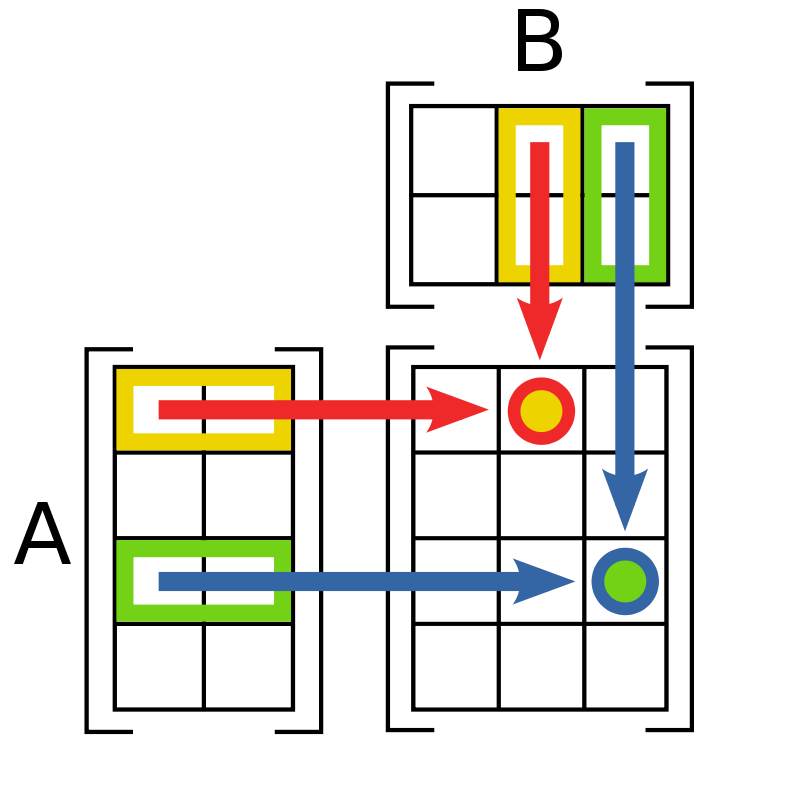
\includegraphics[width=0.5\textwidth]{imagenes/imagenes03/T03IM01.png}
		\caption{Productos de matrices \footnotesize\textit{{(fuente: Wikipedia)}}}
	\end{figure}

\end{defi}
\begin{ejem}.

$A_{3\times 2}=	\left( \begin{matrix}  1&1\\0&-2\\3&4 \end{matrix}\right); \quad 
B_{2\times 4}=\left( \begin{matrix}  1&1&0&-1 \\ 3&3&-1&2 \end{matrix}\right); \quad 
C_{2\times 2}=\left( \begin{matrix}  1&2\\3&4 \end{matrix}\right)$

Calcula, si es posible: 

$A\cdot B; \; A\cdot C; \; B\cdot A;\; B\cdot C;\; C\cdot A; \; C\cdot B; \; A\cdot A; \; B\cdot B; \; C\cdot C $

%\rule{50mm}{0.2pt}

\noindent $A_{3x2}\cdot B_{2x4}=$
\small{$AB_{3x4}=\left( \begin{matrix}  \boxed{1}&\boxed{1}\\0&-2\\3&4 \end{matrix}\right) \cdot \left( \begin{matrix}  \boxed{1}&1&0&-1 \\ \boxed{3}&3&-1&2 \end{matrix}\right)$}\normalsize{$=$}
$\left( \begin{matrix} \boxed{4}&4&-1&1\\-6&-6&2&-4\\15&15&-4&5  \end{matrix}\right)$

\noindent $A_{3x2}\cdot C_{2x2}=AC_{3x2}=$
\small{$\left( \begin{matrix}  1&1\\\boxed{0}&\boxed{-2}\\3&4 \end{matrix}\right) 
\cdot  \left( \begin{matrix}  1&\boxed{2}\\3&\boxed{4} \end{matrix}\right)$}\normalsize{$=$}
$\left( \begin{matrix} 4&6\\-6&\boxed{8}\\15&14  \end{matrix}\right)$

\noindent $\nexists B_{4x2}\cdot A_{3x2}; \quad \nexists B_{4x2}\cdot C_{2x2}; \quad \nexists C_{2x2}\cdot A_{3x2}$

\noindent $C_{2x2}\cdot B_{2x4}=CB_{2x4}$
\small{$=\left( \begin{matrix}  1&2\\\boxed{3}&\boxed{4} \end{matrix}\right) \cdot
\left( \begin{matrix}  1&1&\boxed{0}&-1 \\ 3&3&\boxed{-1}&2 \end{matrix}\right)$}\normalsize{$=$}
$\left( \begin{matrix} 7&7&-2&3\\15&15&\boxed{-4}&5  \end{matrix}
\right)$

\noindent $\nexists A_{3x2} \cdot A_{3x2}; \quad \nexists B_{2x4} \cdot B_{2x4}$

\noindent $C_{2x2} \cdot C_{2x2}=C^2_{2x2}=$
\small{$\left( \begin{matrix}  1&2\\\boxed{3}&\boxed{4} \end{matrix}\right)\cdot \left( \begin{matrix}  1&\boxed{2}\\3&\boxed{4} \end{matrix}\right)$}\normalsize{=}
$\left( \begin{matrix}  7&10\\15&\boxed{22} \end{matrix}\right)$

En este último caso hemos destacado el elemento $2,2$ de $C^2$ como proveniente de multiplicar la fila $2$ de $C$ por la columna $2$ de C. En los otros casos hemos destacados otros elementos a fin de aclarar el producto de matrices. 

\emph{Asegúrese el/la lector/a de que sabe multiplicar matrices antes de continuar}.
\end{ejem}

\begin{prop}{Propiedades del producto de matrices}

\begin{enumerate}

\item El producto de matrices es asociativo: $A\cdot(B\cdot C)=(A\cdot B)\cdot C$
\item !`El producto de matrices es \textbf{no conmutativo}!:  \colorbox{LightYellow}{$\boxed{ \; A\cdot B \neq B\cdot A \; }$}

\vspace{2mm}
$A\cdot B$ puede existir y $B\cdot A$ no. Incluso si existen ambos productos, no tiene por que coincidir. Piénsese en las matrices: $X_{3x1}; \; Y_{1x3}; \; Z_{3x3}$. En que $\exists (ZX)_{3x1}$ pero $\nexists XZ$. Incluso en el caso en que existan ambas, $(XY)_{3x3}\neq (YX)_{1x1}$

Es por ello muy \textbf{importante el orden en que se multiplican las matrices}, llegando a hablar de la matriz que `premultiplica o va delante' y la matriz que `postmultiplica o va detrás'.

\item Distributivas: $\begin{cases} \; A\cdot (B+C)=A\cdot B + A\cdot C \\  \; (A+B)\cdot C=A\cdot C+ B\cdot C   \end{cases}$


\vspace{2mm} !`OJO al orden en que se multiplican las matrices!	


\item Neutro: Matriz Identidad $I_{p\times p}=(i_{kl}) \begin{cases} \; 1 \text{ si } k=l \\ \; 0 \text{ si } k\neq l \end{cases} =$ 
\small{$\left( \begin{matrix} 1 & \cdots & 0 \\ \vdots & \ddots & \vdots \\ 0 & \cdots & 1  \end{matrix}\right)_{p\times p}$}\normalsize{.}

$\forall A_{m \times n}, \; I{n\times n} \therefore \;  A\cdot I=A \quad \wedge \quad \forall A_{m \times n}, \; I{m\times m} \therefore \;  I\cdot A=A $

\item Inversa: esta propiedad, debido a su relevancia, se estudiará en el siguiente apartado.

\vspace{3mm} \textcolor{gris}{$\divideontimes \; (\mathcal M_{n}(\mathbb R) , + , \cdot)\; $ tiene estructura de anillo conmutativo.}
\end{enumerate}
	
\end{prop}
\begin{proof}
La demostración excede de los objetivos del presente texto, por lo que se verá una `comprobación' de las propiedades enunciadas en el  teorema en el apartado de ejercicios.	
\end{proof}

	\begin{figure}[H]
		\centering
		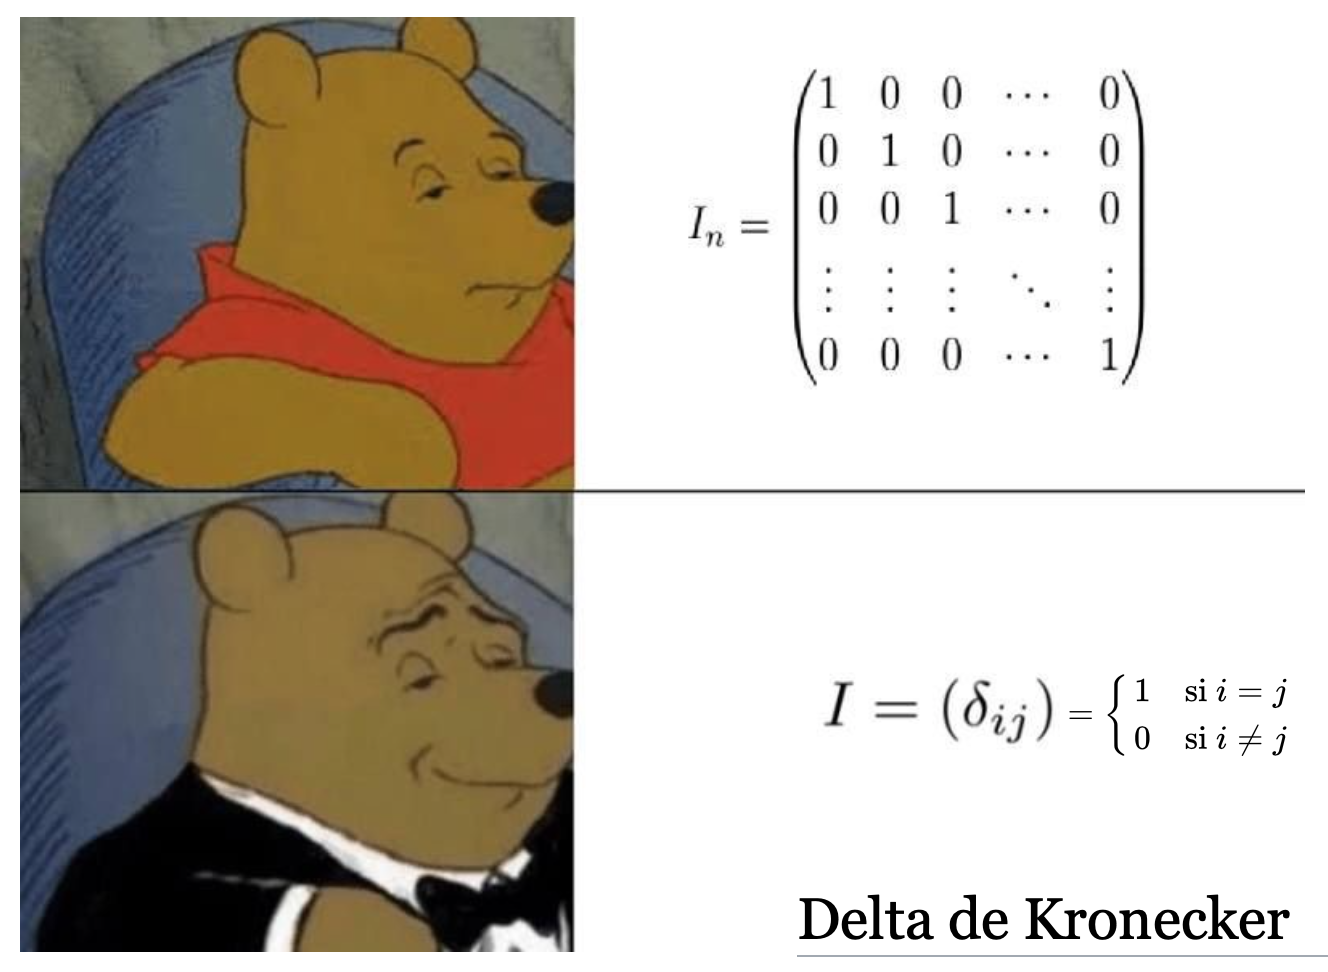
\includegraphics[width=.8\textwidth]{imagenes/imagenes03/T03IM04.png}
	\end{figure}



\begin{coro}
Debido a la `no-conmutatividad' del producto de matrices no se cumplen las llamada identidades notables:

$(A\pm B)^2 \neq A^2 \pm 2 AB + B^2 \quad \wedge \quad (A+B)\cdot (A-B) \neq A^2 - B^2$
\end{coro}
\begin{proof}

Efectivamente: $(A+B)^2=(A+B)\cdot (A+B)=A^2+AB+BA+B^2 \neq A^2 +2AB+ B^2$, puesto que $AB\neq BA$. Lo mismo ocurre con el cuadrado de la resta.

Del	mismo modo: $(A+B)\cdot (A-B)=A^2-AB+BA-B^2 \neq A^2-B^2$, puesto que $AB\neq BA$.  
\end{proof}


\subsection{Potencias de matrices cuadradas}

\begin{defi}
Dada $A\in \mathcal M_n \to A^2=A_{n \times n} \cdot A_{n \times n} =A^2_{n \times n} $

$A^3= \begin{cases}A^2\cdot A=(A\cdot A )\cdot A  \\ A \cdot A^2 = A\cdot (A \cdot A)\end{cases}$	

Evidentemente, las sucesivas potencias de una matriz cuadrada conmutan, es decir, podemos calcular $A^8=A^5 \cdot A^3$ o $A^3\cdot A^5$.

\noindent \small{Así, en general, podríamos definir (`por inducción' - ver apéndice \ref{inducción})} $A^n=A\cdot A \cdots \cancelto{n \text{ veces }}{.}  \cdot A$\normalsize{.}
\end{defi}

\begin{ejem}
Calcula las potencias enésimas de: 

$M=\left( \begin{matrix} 1&2\\0&1 \end{matrix} \right) \quad N=\left( \begin{matrix} 1&1/5&1/5 \\ 0&1&0 \\ 0&0&1 \end{matrix} \right)$

$M=\left( \begin{matrix} 1&2\\0&1 \end{matrix} \right) \to M^2=MM=\left( \begin{matrix} 1&2\\0&1 \end{matrix} \right) \cdot \left( \begin{matrix} 1&2\\0&1 \end{matrix} \right) =\left( \begin{matrix} 1&4\\0&1 \end{matrix} \right) \to M^3=M^2\cdot M= \left( \begin{matrix} 1&6\\0&1 \end{matrix} \right) \to M^4=\left( \begin{matrix} 1&8\\0&1 \end{matrix} \right) \Rightarrow  \; M^n=\left( \begin{matrix} 1&2n\\0&1 \end{matrix} \right)\;  $ 

Realmente, hemos obtenido una `conjetura'. Ahora deberíamos someterla a la prueba del `método de inducción completa'.

$N=\left( \begin{matrix} 1&1/5&1/5 \\ 0&1&0 \\ 0&0&1 \end{matrix} \right) \to N^2=\left( \begin{matrix} 1&2/5&2/5 \\ 0&1&0 \\ 0&0&1 \end{matrix} \right) \to N^3=\left( \begin{matrix} 1&3/5&3/5 \\ 0&1&0 \\ 0&0&1 \end{matrix} \right)\to N^4=\left( \begin{matrix} 1&4/5&4/5 \\ 0&1&0 \\ 0&0&1 \end{matrix} \right) \Rightarrow \; N^n=\left( \begin{matrix} 1&n/5&n/5 \\ 0&1&0 \\ 0&0&1 \end{matrix} \right)\; $

De nuevo, este resultado solo es una conjetura.
	
\end{ejem}


\subsection{Matriz Inversa}

\begin{defi}

Dada $A\in \mathcal M_{n\times n} (\mathbb R)$, una matriz cuadrada, puede que exista otra matriz cuadraba $B_{n\times n}$ de modo que:

$A_{n\times n}\cdot B_{n \times n}= B_{n\times x}\cdot A_{n \times n}=I_n$, con $I_n=I_{n\times n}$, la identidad de orden $n$.

Si esto ocurre, si $\exists B$, decimos que $B$ es la inversa de $A$ y la representamos por $A^{-1}$, es decir:




\begin{myblock}{Matriz inversa}
\vspace{2mm} $\forall A\in \mathcal M_{n\times n} (\mathbb R), \; \text{ si } \exists A^{-1}\in \mathcal M_{n\times n} (\mathbb R) \; \therefore \; $

\vspace{3mm} \centerline{$\boxed{\; A\cdot A^{-1}=A^{-1}\cdot A=I\; }\; $,} 

\vspace{2mm} decimos que $A$ es `invertible o regular' y que $A^{-1}$ es su matriz inversa. 
\end{myblock}

\end{defi}

\noindent \textbf{Observaciones:}

Para tener matriz inversa, la matriz de partida ha de ser cuadrada. Pero no todas las matrices cuadradas tienen inversa. Cuando una matriz cuadrada no tiene inversa de dice que es una `matriz singular o no invertible'.

Por ejemplo, la matriz $\left( \begin{matrix} 1&0\\0&0  \end{matrix}\right)$ es singular, pues no existe ninguna matriz $\left( \begin{matrix} a&b\\c&d  \end{matrix}\right)$ tal que $ \left( \begin{matrix} 1&0\\0&0  \end{matrix}\right)\cdot \left( \begin{matrix} a&b\\c&d  \end{matrix}\right)  =\left( \begin{matrix}1&0\\0&1   \end{matrix}\right)=I$ (\textit{Compruébese resolviendo el SEL})

En el próximo capítulo, `Determinantes', veremos un teorema que asegura cuando una matriz cuadrada tiene o no inversa.

\subsection{Propiedades interesantes de las operaciones con matrices}

\begin{lema}
\label{lema1}\label{producto-traspuestas}

$(A+B)^T=A^T + B^T\; $ La traspuesta de la suma de matrices es la suma de matrices traspuestas.
\end{lema}
\begin{proof}

Sea $A_{m\times n}=(a_{ij}); \; B_{m \times n}=(b_{ij}) \to A^T=(a_{ji})\; \wedge \; B^T=(b_{ji})$

Como $A+B=	(a_{ij}+b_{ij}) \to (A+B)^T=(a_{ji}+b_{ji})=(a_{ji}) + (b_{ji})=B^T+A^T$ 

\end{proof}



\begin{teor}
$\divideontimes \; \; $ Toda matriz cuadrada $M$ se puede descomponer como suma de dos matrices cuadradas $S$ y $H$, una de ellas simétrica y la otra antisimétrica.	
\end{teor}
\begin{proof}
Basta con considerar $S=\frac 1 2 (M+M^T)$ y $H=\frac 1 2 (M-M^T)$

En efecto, $S+T = \frac 1 2 [ (M+M^T)+(M-M^T)]= \frac 1 2 2M= M$

Además, $S^T = \frac 1 2 (M+M^T)^T=\frac 1 2 (M^T+M)=S\; $ Simétrica.

Y, $\; H^T=\frac 1 2 (M-M^T)^T=\frac 1 2 (M^T-M)=-\frac 1 2 (M-M^T)=-H\;$, Antisimétrica.

Hemos usado para demostración la proposición \ref{propo1} ($(A^T)^T=A)$) y el lema anterior \ref{lema1}.
\end{proof}
\begin{teor}
$\divideontimes \; \; $ La traspuesta del producto de dos matrices cuadradas es igual al producto de las matrices transpuestas, pero con el orden de multiplicación invertido. $(\; A\cdot B)^T=B^T \; \cdot \; A^T$ 	
\end{teor}
\begin{proof}

La demostración es más complicada en este caso, así que, para mayor claridad en la exposición, nos contentaremos con una `comprobación' para un caso particular, que no es ninguna demostración pero será suficiente para los objetivos de este libro. 	

$A=\left( \begin{matrix} 1&0 \\ 2&-1   \end{matrix}\right); \qquad B=\left( \begin{matrix} 3&-2&1&0 \\-2&1&1&-1  \end{matrix}\right)$


$A\cdot B=\left( \begin{matrix} 1&0 \\ 2&-1  \end{matrix}\right) \cdot  \left( \begin{matrix} 3&-2&1&0\\-2&1&1&-1  \end{matrix}\right) = \left( \begin{matrix} 3&2&-1&0\\8&-5&1&1 \end{matrix}\right) \to$

$ (AB)^T=\; \left( \begin{matrix} 3&8\\2&-5\\-1&1\\0&1 \end{matrix}\right)\; $

$B^T\cdot A^T=\left( \begin{matrix} 3&-2\\-2&1\\1&1\\0&-1 \end{matrix}\right) 
\cdot \left( \begin{matrix} 1&2\\0&-1  \end{matrix}\right)=
\; \left( \begin{matrix}   3&8\\2&-5\\-1&1\\0&1 \end{matrix}\right)\; $


Destacar que está curiosa propiedad (se alterna el orden) ya vimos que se cumplía con una operación no-conmutativa como la composición de funciones y el cálculo de la función inversa: $(f \circ g)^{-1}= g^{-1} \circ f^{-1}$

\end{proof}
\begin{teor}
\label{prod-inv}
$\divideontimes \; \;$ La inversa del producto de dos matrices es igual al producto de las matrices inversas, pero con el orden de multiplicación invertido. $ \; (A\cdot B)^{-1}=B^{-1} \; \cdot \; A^{-1}$ 	


	
\end{teor}
\begin{proof}

De modo análogo al teorema anterior, la demostración excede a los objetivos de este curso y solo haremos una mera comprobación que veremos en el apartado de ejercicios, después de aprender a calcular matrices inversas por el método de Gauss.

De nuevo se cumple la curiosa propiedad antes comentada.


\end{proof}

\begin{teor}
	$(A^{-1})^{-1}=A\; \qquad (A^T)^{-1}=(A^{-1})^T$
\end{teor}
\begin{proof}
El mismo comentario que en el teorema anterior, veremos `comprobaciones' en ls ejercicios.	
\end{proof}




\section{Método de Gauss para el cálculo de $A^{-1}$}


Supongamos que la matriz tiene inversa $\; A= \left( \begin{matrix}  a_{11}&a_{12}&\cdots &a_{1n}\\ a_{21}&a_{22}&\cdots &a_{2n}\\ \vdots&\vdots&\ddots&\vdots\\a_{n1}&a_{n2}&\cdots &a_{nn}  \end{matrix} \right)$

El método de Gauss-Jordan consiste, esquemáticamente en colocar en la misma matriz a $A$, una barra separadora y detrás a la matriz $I$. Conseguir, mediante transformaciones de Gauss que primero por debajo de la diagonal principal y después por arriba de ésta, todos los elementos que habían en $A$ sean ceros, diagonalizar la matriz $A$ mediante transformaciones de Gauss. Luego, dividiendo cada fila por la cantidad correspondiente, obtener, donde estaba $A$, que esté la matriz Identidad $I$. Si ello ha sido posible, la matriz que haya quedado detrás de la barra inicial será la matriz inversa $A^{-1}$.

Lo que no está permitido ahora /en SEL sí lo estaba) es cambiar de posición ni filas ni columnas.

El método de Gauss permite obtener $A^{-1}$ si ello es posible, si no lo es se llega a un paso a partir del cual no se puede continuar el proceso, por ello, no es éste el mejor método para el cálculo de inversas pero no podremos usar un método mejor (por `adjuntos') hasta que desarrollemos el siguiente tema de determinantes.

\vspace{3mm}

\centerline{$\colorbox{LightYellow}{\boxed{ \; \; [\; A \; | \; I \; ] \; \to \text{ transf. Gauss } \to  \; [\; I \; | \; \boldsymbol{ A^{-1} } \; ] \; \; }}$}
\justify


$\left[ \begin{matrix}  a_{11}&a_{12}&\cdots &a_{1n}\\ a_{21}&a_{22}&\cdots &a_{2n}\\ \vdots&\vdots&\ddots&\vdots\\a_{n1}&a_{n2}&\cdots &a_{nn}  \end{matrix} \right|
 \left. \begin{matrix} 1&0&\cdots&0\\ 0&1&\cdots&0\\  \vdots&\vdots&\ddots&\vdots \\0&0&\cdots&1    \end{matrix}   \right] \to
  \left[ \begin{matrix} 1&0&\cdots&0\\ 0&1&\cdots&0\\  \vdots&\vdots&\ddots&\vdots \\0&0&\cdots&1    \end{matrix}   \right|
  \left. \begin{matrix} * & * & \cdots & * \\  * & * & \cdots & * \\  \vdots&\vdots&\ddots&\vdots    \\ * & * & \cdots & * \\   \end{matrix} \right]$


Si se ha conseguido escribir delante la matriz $I$, la matriz que figura detrás (*) será la inversa de $A$, $\; A^{-1}$

\begin{ejem}
Calcula, si es posible, las siguientes matrices inversas:

$A=\left[\begin{matrix} 4&-2\\2&1  \end{matrix}\right]; \quad 
B=\left[\begin{matrix} 1&0&2\\3&1&-1\\-2&1&5  \end{matrix}\right] \quad 
C=\left[\begin{matrix} 4&6\\2&3  \end{matrix}\right]$

%\vspace{2mm}
\rule{5cm}{0.2pt}

%\vspace{2mm}

--- Inversa de A:

$A=\left[\begin{matrix} 4&-2\\2&1  \end{matrix}\right|
\left. \begin{matrix}1&0\\0&1\end{matrix} \right] \to (\; F2\to 2F2-F1\;) \to 
\left[\begin{matrix} 4&-2\\0&4  \end{matrix}\right|
\left. \begin{matrix}1&0\\-1&2\end{matrix} \right] \to 
(\;F1\to 2F1+F2 \;) \to 
\left[\begin{matrix} 8&0\\0&4  \end{matrix}\right|
\left. \begin{matrix}1&2\\-1&2\end{matrix} \right] \to \begin{cases} \; F1\to F1/8 \\ F2\to F2/4\end{cases} \to $

$\to \left[\begin{matrix} 1&0\\0&1  \end{matrix}\right|
\left. \begin{matrix}1/8&1/4\\-1/4&1/2\end{matrix} \right]$ Como delante está $I \Rightarrow $

$A^{-1}=\left[ \begin{matrix}1/8&1/4\\-1/4&1/2\end{matrix} \right]=\dfrac 1 8 \left[ \begin{matrix}1&2\\-1&4\end{matrix} \right]$

Comprobémoslo: $A\cdot A^{-1} = I = A^{-1}\cdot A$:

$A\cdot A^{-1} = \left[\begin{matrix} 4&-2\\2&1  \end{matrix}\right] \cdot \dfrac 1 8 \left[ \begin{matrix}1&2\\-1&4\end{matrix} \right] = $
$\dfrac 1 8 \left [ \begin{matrix} 8&0\\0&8 \end{matrix} \right]=I$


$A^{-1} \cdot A =   \dfrac 1 8 \left[ \begin{matrix}1&2\\-1&4\end{matrix} \right] \cdot \left[\begin{matrix} 4&-2\\2&1  \end{matrix}\right]=$
$\dfrac 1 8 \left [ \begin{matrix} 8&0\\0&8 \end{matrix} \right]=I$

Luego, efectivamente, la inversa de $A$ es: $ \; A^{-1}=\dfrac 1 8 \left[ \begin{matrix}1&2\\-1&4\end{matrix} \right] \; $

--- Inversa de B:




\noindent \small{
$\left[\begin{matrix} 1&0&2\\3&1&-1\\-2&1&5  \end{matrix}\right|
\left. \begin{matrix} 1&0&0 \\ 0&1&0 \\0&0&1  \end{matrix} \right] \to \begin{cases} F2\to F2+2F1 \\ F3\to F3-3F1   \end{cases} \to $	
$\left[\begin{matrix} 1&0&2\\0&1&-7\\0&1&9  \end{matrix}\right|
\left. \begin{matrix} 1&0&0 \\ -3&1&0 \\2&0&1  \end{matrix} \right] \to $}

\noindent \small{$(\;F3\to F3-F2 \; )  \to 
\left[\begin{matrix} 1&0&2\\0&1&-7\\0&0&16  \end{matrix}\right|
\left. \begin{matrix} 1&0&0 \\ -3&1&0 \\5&-1&1  \end{matrix} \right] \to 
\begin{cases}\; F1\to 8F1-F3 \\ \; F2\to 16F2+7F3  \end{cases}\to  $}

\noindent \small{$  \to   
\left[\begin{matrix} 8&0&0\\0&16&0\\0&0&16  \end{matrix}\right|
\left. \begin{matrix} 3&1&-1 \\ -13&9&7 \\5&-1&1  \end{matrix} \right]
* \; (F1\to 2F1) \;  *  
\left[\begin{matrix} 16&0&0\\0&16&0\\0&0&16  \end{matrix}\right|
\left. \begin{matrix} 6&2&-2 \\ -13&9&7 \\5&-1&1  \end{matrix} \right]
$}  

\normalsize{Como delante, previo a dividir por $16$ cada una de las filas, aparecerá la matriz identidad, la matriz de atrás es la inversa de B}:

\hspace{15mm} $\; B^{-1}= \dfrac 1 {16} \left[ \begin{matrix} 6&2&-2 \\ -13&9&7 \\5&-1&1  \end{matrix} \right]\; $

Compruébese que realmente se trata de la inversa de $B$, calculando: $B\cdot B^{-1}=B^{-1}\cdot B=I$

--- Inversa de C:

$\left[\begin{matrix} 4&6\\2&3  \end{matrix}\right|
\left.\begin{matrix} 1&0\\0&1  \end{matrix}\right] \to (F2\to 2F2-F1) \to 
\left[\begin{matrix} 4&\boxed{6}\\0&0  \end{matrix}\right|
\left.\begin{matrix} 1&0\\-1&2  \end{matrix}\right]$

\noindent \small{Es imposible combinar la $F1$ con la $F2$ para conseguir que $c_{12}=0 \to \; \nexists \;  C^{-1} \; $}\normalsize{.} 
\end{ejem}


\newpage %****************************************************
\section{Aplicaciones de las matrices}


\begin{myexampleblock}{Aplicaciones de las matrices}
	
Una vez que ya conocemos a fondo las matrices, puesto que hemos visto los distintos tipos que hay y las operaciones que podemos realizar con ellas. Vamos a ver sus aplicaciones, ya que las matrices son una herramienta muy útil no sólo en el campo de las matemáticas y la física como era de esperar; sino también en el campo de las ciencias sociales, por ejemplo en economía y en geografía. Esta gran utilidad se debe a que las matrices aportan un nuevo lenguaje facilitando el trabajo en una gran cantidad de ámbitos.

Empezaremos en primer lugar con las aplicaciones en \textbf{Matemáticas}, donde vamos a distinguir las aplicaciones en las distintas ramas:

--- Álgebra lineal: 

1. En esta rama destaca la utilidad en la resolución de sistemas de ecuaciones de la forma AX = B, mediante el cálculo de la matriz inversa (siguiente tema $\; X=A^{-1}\cdot B\; $).

2. Estudio de las aplicaciones lineales entre dos espacios vectoriales mediante la matriz asociada, que nos permite calcular el núcleo y la imagen (temas siguientes de ampliación de conocimientos $\divideontimes$).

---Análisis:

$\divideontimes$ En la rama del análisis se utilizan las matrices jacobianas, que se usan para expresar las derivadas parciales de una función en varias variables. Si f(x,y,z) está definida de la siguiente forma: 

$f:\mathbb R^2 \to \mathbb R^3 \Rightarrow J=\left(\begin{matrix} \dfrac{\partial f_1}{\partial x}  &\dfrac{\partial f_1}{\partial y}&\dfrac{\partial f_1}{\partial z} \\ \dfrac{\partial f_2}{\partial x} &\dfrac{\partial f_2}{\partial y} &\dfrac{\partial f_3}{\partial z}  \end{matrix}\right)$

--- Probabilidad: 

Cadenas de Markov: un tipo especial de proceso estocástico discreto en el que la probabilidad de que ocurra un evento depende solamente del evento inmediatamente anterior.

--- En teoría de grafos las matrices son de gran utilidad y tienen aplicaciones en diversas ramas del conocimiento humano (demografía, sociología, etc.)


Continuamos con las aplicaciones en la \textbf{Física}. (Relatividad Especial $\divideontimes$) La aplicación más importante en este campo son las transformaciones de Lorentz, que dan las ecuaciones del movimiento de un punto en línea recta y sobre el plano conocida la velocidad de la luz.

Por ejemplo: suponiendo que el punto se desplaza sobre el eje $OX$ y que estamos en un espacio tetradimensional, donde la cuarta dimensión es el tiempo, entonces, el punto tendrá como coordenadas iniciales $(x,y,z,t)$ y como finales $(x’,y’,z’,t’)$. Las ecuaciones que dan esta transformación son:

$\left( \begin{matrix} x', \; t'  \end{matrix} \right) =$
$\left( 
\begin{matrix}  \dfrac {1}{\sqrt{1- \left( \dfrac v c \right)^2}}  &\dfrac {-v}{\sqrt{1- \left( \dfrac v c \right)^2}}  \\ \dfrac {-v/c^2}{\sqrt{1- \left( \dfrac v c \right)^2}} &\dfrac {1}{\sqrt{1- \left( \dfrac v c \right)^2}} \end{matrix}
 \right)$
$ \cdot \left( \begin{matrix}  x \\ t \end{matrix} \right); \; \quad y'=y; \; z'=z$

Donde c representa la velocidad de la luz.


Una vez que ya hemos visto algunas de las aplicaciones más importantes en Ciencias, vamos a ver la importancia que tienen en las \textbf{Ciencias Sociales}, como la \textbf{Economía.}

Las matrices se utilizan para la presentación de datos de un problema en forma de tabla de doble entrada. Un ejemplo de esto es el modelo Input-Output, que permite solucionar problemas macroeconómicos (matriz de Leontiev), algunos de los cuáles son: orientar o estructurar los sectores productivos, poder predecir las demandas de producción, interpretar las relaciones económicas existentes entre los distintos sectores de producción.

Si continuamos por la Geografía, también aparecen cuando hay tablas de doble entrada, por ejemplo, para hacer referencia a la distancia que hay entre varias ciudades. En comunicaciones aéreas, para ver las distintas formas de interconectar vuelos entre diferentes paises. Etc.

\end{myexampleblock}






\begin{figure}[H]
	\centering
	
\includegraphics[width=1\textwidth]{imagenes/imagenes03/T03IM02.png}
\end{figure}









\section {Ejercicios}
\subsection {Ejercicios resueltos}

\begin{ejre}
	Escribe una matriz cuadrada de orden $3$ cuyos elementos cumplan: $\begin{cases}  2j-i & \text{ si } \textcolor{blue}{i \le j} \\ (-1)^{i+j} & \text{ si } \textcolor{red}{i>j}  \end{cases}$
\end{ejre}

\begin{proofw}\renewcommand{\qedsymbol}{$\diamond$}

\hspace{10mm}$\left( 
\begin{array}{ccc} \textcolor{blue}{a_{11}} & \textcolor{blue}{a_{12}} & \textcolor{blue}{a_{13}} \\
 \textcolor{red}{a_{21}} & \textcolor{blue}{a_{22}} & \textcolor{blue}{a_{23}} \\
\textcolor{red}{a_{31}} & \textcolor{red}{a_{32}} & \textcolor{blue}{a_{33}}
\end{array} \right) 
\to \; \left( \begin{array} {ccc}
1 &3 &5 \\-1 & 2 & 4 \\ 1 & -a & 3  	
\end{array} \right)$

	
\end{proofw}


\begin{ejre}
Considera las matrices:  

$ M=\left( \begin{matrix} 1&-1&2\\-2&0&3  \end{matrix} \right)\; \quad  N=\left( \begin{matrix} 3&-1&0\\1&2&1  \end{matrix} \right)\; \quad  P=\left( \begin{matrix}  2&-1\\3&1\\-2&0 \end{matrix} \right)$

\noindent Calcula: 
$\; \; a) \; M+N \quad b)\; \frac 2 5 N; \quad c)\; -M; \quad d)\; \frac 1 2 M - 3 N$
 
 $e)\; 2M-3P^T; \quad f)\; 3(N^T+P)-M^T\quad g)\; MP \neq PM$

 $ h) (MN^T)P^T=M(N^TP^T); \quad i) \; P(M+N)=PM+PN$

 $j)\; (MP)^T=P^TM^T; \quad i)\; MI=M \text { y } IM=M $
\end{ejre}
\begin{proofw}\renewcommand{\qedsymbol}{$\diamond$}

--- a) $M+N=\left( \begin{matrix} 1&-1&2\\-2&0&3  \end{matrix} \right)\; + \;\left( \begin{matrix} 3&-1&0\\1&2&1  \end{matrix} \right) = 
\left( \begin{matrix} 4&-2&2\\-1&2&4  \end{matrix} \right)$

\noindent --- b) $\frac 2 5 N = \frac 2 5 \; \left( \begin{matrix} 3&-1&0\\1&2&1  \end{matrix} \right) =\left( \begin{matrix} 6/5&-2/5&0\\2/5&4/5&2/5  \end{matrix} \right)$

\noindent --- c) $-M=-\; \left( \begin{matrix} 1&-1&2\\-2&0&3  \end{matrix} \right) =\left( \begin{matrix} -1&1&-2\\2&0&-3  \end{matrix} \right)$

\noindent --- d) $\frac 1 2 M -2N=\frac 1 2 \; \left( \begin{matrix} 1&-1&2\\-2&0&3  \end{matrix} \right) - 2 \; \left( \begin{matrix} 3&-1&0\\1&2&1  \end{matrix} \right)= $

\noindent $=\left( \begin{matrix} 1/2&-1/2&1\\-1&0&3/2  \end{matrix} \right)-
\left( \begin{matrix} 9&-3&0\\3&6&3  \end{matrix} \right)=
\left( \begin{matrix} -17/2&5/2&1\\-4&-6&-3/2  \end{matrix} \right) $

\noindent --- e) $2M-3P^T=2\; \left( \begin{matrix} 1&-1&2\\-2&0&3  \end{matrix} \right) - 3\; \left( \begin{matrix} 2&3&-2\\-1&1&0  \end{matrix} \right)=$

\noindent $\left( \begin{matrix} 2&-2&4\\-4&0&6   \end{matrix} \right) - \left( \begin{matrix} 6&0&-6\\3&6&3   \end{matrix} \right) = 
\left( \begin{matrix}  -4&-11&10\\-1&-3&6  \end{matrix} \right)$

\noindent --- f) $3(N^T+P)-M^T=3\left( 
\left( \begin{matrix}  3&1\\-1&2\\01  \end{matrix} \right)+
\left( \begin{matrix}  2&-1\\3&1\\-2&0  \end{matrix} \right)
  \right) - 
\left( \begin{matrix} 1&-2\\-1&0\\2&3   \end{matrix} \right) =$

\noindent $3\; \left( \begin{matrix}   5&0\\2&3\\-2&1 \end{matrix} \right)
- \left( \begin{matrix} 1&-2\\-1&0\\2&3   \end{matrix} \right)=
\left( \begin{matrix} 15&0\\6&9\\-6&3   \end{matrix} \right)-
\left( \begin{matrix} 1&-2\\-1&0\\2&3   \end{matrix} \right)=
\left( \begin{matrix} 14&2\\7&9\\-8&0   \end{matrix} \right)$

\noindent --- g) $MP=\left( \begin{matrix} 1&-1&2\\-2&0&3  \end{matrix} \right) \cdot \left( \begin{matrix}  2&-1\\3&1\\-2&0 \end{matrix} \right) =
\left( \begin{matrix} -5&-2\\-8&2   \end{matrix} \right) $

\noindent $PM=\left( \begin{matrix}  2&-1\\3&1\\-2&0 \end{matrix} \right) \cdot \left( \begin{matrix} 1&-1&2\\-2&0&3  \end{matrix} \right)  =
\left( \begin{matrix} 4&-2&1\\1&-3&9\\-2&2&-4  \end{matrix} \right) \neq MP$

\noindent --- h) $(MN^T)P^T=\left[ 
\left( \begin{matrix} 1&-1&2\\-2&0&3    \end{matrix} \right)  \cdot  
\left( \begin{matrix} 3&1\\-1&2\\0&1   \end{matrix} \right)  \right] \cdot 
\left( \begin{matrix} 2&3&2\\-1&1&0   \end{matrix} \right) = $

\noindent $\left( \begin{matrix} 4&1 \\ -6&1   \end{matrix} \right)\cdot \left( \begin{matrix} 2&3&2\\-1&1&0   \end{matrix} \right) = 
\left( \begin{matrix}  7&13&8\\-13&-17&-12  \end{matrix} \right)$

\noindent $M(N^TP^T)= \left( \begin{matrix} 1&-1&2\\-2&0&3   \end{matrix} \right) \cdot \left[
\left( \begin{matrix} 3&1\\-1&2\\0&1   \end{matrix} \right)
\cdot \left( \begin{matrix} 2&3&2\\-1&1&0   \end{matrix} \right)
\right] =$

\noindent $\left( \begin{matrix} 1&-1&2\\-2&0&3   \end{matrix} \right) \cdot
\left( \begin{matrix} 5&10&6\\ -4&-1&-2\\-1&1&0   \end{matrix} \right) = 
\left( \begin{matrix} 7&13&8\\-13&-17&-12   \end{matrix} \right) = (MN^T)P^T$

\small{\noindent --- i) $P(M+N)=
\left( \begin{matrix} 2&-1\\3&1\\2&0   \end{matrix} \right) \cdot
\left [
\left( \begin{matrix}  1&-1&2\\-2&0&3  \end{matrix} \right)  + 
\left( \begin{matrix} 3&-1&0\\1&2&1   \end{matrix} \right) 
\right]=$}

\small{\noindent $\left( \begin{matrix} 2&-1\\3&1\\2&0   \end{matrix} \right)  \cdot \left( \begin{matrix}  4&-2&2\\ -1&2&4  \end{matrix} \right) =
\left( \begin{matrix}  9&-6&0\\11&-4&10\\8&-4&4  \end{matrix} \right) $}



\small{\noindent $PM+PN= \left( \begin{matrix} 2&-1\\3&1\\2&0   \end{matrix} \right)\cdot \left( \begin{matrix} 1&-1&2\\-2&0&3   \end{matrix} \right) +
   \left( \begin{matrix} 2&-1\\3&1\\2&0   \end{matrix} \right)
   \cdot \left( \begin{matrix}  3&-1&0\\1&2&1  \end{matrix} \right) =$}
   
 \small{\noindent $\left( \begin{matrix}  4&-2&1\\1&-3&9\\2&-2&4   \end{matrix} \right) 
   +\left( \begin{matrix} 5&-4&1\\10&-1&1\\6&-2&0  \end{matrix} \right) 
   =
   \left( \begin{matrix} 9&-6&2\\11&-4&10\\8&-4&4   \end{matrix} \right) 
   =P(M+N)$}\normalsize{.}

   
   \noindent --- j) $M_{2\times 3}\cdot I_{3\times 3}= \left( \begin{matrix} 1&-1&2\\-2&0&3   \end{matrix} \right) \cdot 
   \left( \begin{matrix} 1&0&0\\0&1&0\\0&0&1 \end{matrix} \right) = \left( \begin{matrix} 1&-1&2\\-2&0&3   \end{matrix} \right)=M$
   
   \noindent $I_{2\times 2}\cdot M_{2\times 3}=\left( \begin{matrix} 1&0\\0&1 \end{matrix} \right) \cdot \left( \begin{matrix} 1&-1&2\\-2&0&3   \end{matrix} \right)=\left( \begin{matrix} 1&-1&2\\-2&0&3   \end{matrix} \right) =M$

\end{proofw}

\begin{ejre}.

\noindent Sean $A= \left( \begin{matrix}  9&1&1\\1&2&1\\1&18&1 \end{matrix} \right); \quad B=\left( \begin{matrix}  1&1\\1&1\\1&1 \end{matrix} \right); \quad C=\left( \begin{matrix} 10&2&2\\2&3&3\\2&19&2  \end{matrix} \right)$. Calcula:
	
\small{ \noindent  $a)\; AB;\; \; b)\; B^TA^T;\; \;  c)\; (AB)^T;\; \; d)\; (A+I)^2; \; \;  e)\; (A-C)^2;\; f)\; \; A^2-2AC+C^2$}\normalsize{.}
\end{ejre}
\begin{proofw}\renewcommand{\qedsymbol}{$\diamond$}

\noindent	--- a) $AB=\left( \begin{matrix}  9&1&1\\1&2&1\\1&18&1 \end{matrix} \right) \cdot \left( \begin{matrix}  1&1\\1&1\\1&1 \end{matrix} \right) = \left( \begin{matrix} 11&11\\4&4\\20&20  \end{matrix} \right)$ 

\noindent --- b) y c)  $B^TA^T=(AB)^T=\left( \begin{matrix}11&4&20\\11&4&20  \end{matrix} \right)$ 

\noindent --- d) $(A+I)^2\to (A+I)= \left( \begin{matrix}  9&1&1\\1&2&1\\1&18&1 \end{matrix} \right) +  \left( \begin{matrix}  1&0&0\\0&1&0\\0&08&1 \end{matrix} \right)=
 \left( \begin{matrix}  10&1&1\\1&3&1\\1&18&2 \end{matrix} \right)$
 
 \noindent $(A+I)^2=  \left( \begin{matrix}  10&1&1\\1&3&1\\1&18&2 \end{matrix} \right) \cdot  \left( \begin{matrix}  10&1&1\\1&3&1\\1&18&2 \end{matrix} \right) =
  \left( \begin{matrix}  102&31&13\\16&27&8\\30&91&23 \end{matrix} \right)$
  
  
  \noindent --- e) $(A-C)^2 \to A-C= \left( \begin{matrix}  9&1&1\\1&2&1\\1&18&1 \end{matrix} \right)-\left( \begin{matrix} 10&2&2\\2&3&3\\2&19&2  \end{matrix} \right)=$
  $\left( \begin{matrix} -1&-1&-1\\-1&-1&-2\\-1&-1&-1  \end{matrix} \right)$
  
  \noindent $(A-C)^2=\left( \begin{matrix} -1&-1&-1\\-1&-1&-2\\-1&-1&-1  \end{matrix} \right) \cdot \left( \begin{matrix} -1&-1&-1\\-1&-1&-2\\-1&-1&-1  \end{matrix} \right)=
  \left( \begin{matrix} 3 & 3& 4\\4 & 4& 5\\ 3& 3& 4  \end{matrix} \right)$

\noindent --- f) $A^2-2AC+C^2= 
\left( \begin{matrix}  9&1&1\\1&2&1\\1&18&1 \end{matrix} \right)\cdot \left( \begin{matrix}  9&1&1\\1&2&1\\1&18&1 \end{matrix} \right)
-2\left( \begin{matrix}  9&1&1\\1&2&1\\1&18&1 \end{matrix} \right)\cdot
\left( \begin{matrix} 10&2&2\\2&3&3\\2&19&2  \end{matrix} \right)+
\left( \begin{matrix} 10&2&2\\2&3&3\\2&19&2  \end{matrix} \right)\cdot \left( \begin{matrix} 10&2&2\\2&3&3\\2&19&2  \end{matrix} \right)=\cdots = 
\left( \begin{matrix}  3&13&-5\\10&20&2\\-6&4&-14 \end{matrix} \right)\neq (A-C)^2$

\end{proofw}

\begin{ejre} Realiza todos los productos posibles.
		
\noindent \small{$M=\left( \begin{matrix} 1\\-1\\2\\-2   \end{matrix} \right); \quad N=\left( \begin{matrix}  2&\;3&\;0&\;1  \end{matrix} \right); \quad P=\left( \begin{matrix} 1&2&1&-1 \\0&-2&1&1\\3&1&-1&1\\3&0&-1&1   \end{matrix} \right)$}\normalsize{.}

\end{ejre}

\begin{proofw}\renewcommand{\qedsymbol}{$\diamond$}


$MN=\left( \begin{matrix}  2&3&0&1\\-2&-3&0&-1\\4&6&0&2\\-4&-6&0&-2  \end{matrix} \right)$ $\qquad$ 
$NM=(-3)$ $\qquad$ 
$\nexists MP$ 

$PM=\left( \begin{matrix}  3\\2\\-2\\-1  \end{matrix} \right)$
$\qquad$ 
$NP=(5\quad -2\quad 4\quad 2)$ $\qquad$
$\nexists PN$


\end{proofw}


\begin{ejre}
	Considera $A=\left( \begin{matrix} 1&2&3\\4&5&6\\7&8&9 \end{matrix} \right)$. Descompón A como suma de dos matrices, una $S$ simétrica y una $H$ antisimétrica.
\end{ejre}
\begin{proofw}\renewcommand{\qedsymbol}{$\diamond$}.

$S=\frac 1 2 (A+A^t)= \frac 1 2 \left [\left( \begin{matrix} 1&2&3\\4&5&6\\7&8&9 \end{matrix} \right) + \left( \begin{matrix} 1&4&7\\2&5&8\\3&6&9 \end{matrix} \right) \right] = \frac 1 2  \left( \begin{matrix} 2&6&10\\6&10&14\\10&14&18 \end{matrix} \right) =  \left( \begin{matrix} 1&3&5 \\3&5&7\\5&7&9 \end{matrix} \right)\; $ Con $S^T=S$, simétrica.
 
$H=\frac 1 2 (A-A^t)= \frac 1 2 \left [\left( \begin{matrix} 1&2&3\\4&5&6\\7&8&9 \end{matrix} \right) - \left( \begin{matrix} 1&4&7\\2&5&8\\3&6&9 \end{matrix} \right) \right] =
 \frac 1 2  \left( \begin{matrix} 0&-2&-4\\2&0&-2\\4&2&0 \end{matrix} \right) =  \left( \begin{matrix} 0&-1&-2 \\1&0&-1\\2&1&0 \end{matrix} \right)
\; $ con $H^T=-H$, antisimétrica. 

$ S+H= \left( \begin{matrix} 1&3&5 \\3&5&7\\5&7&9 \end{matrix} \right)  + \left( \begin{matrix} 0&-1&-2 \\1&0&-1\\2&1&0 \end{matrix} \right) =  \left( \begin{matrix} 1&2&3 \\4&5&6\\7&8&9 \end{matrix} \right) =A$
	
\end{proofw}


\begin{ejre}
Calcula $a$, $b$ y $c$ en la expresión:

$\quad$

$3\left( \begin{matrix} 3&b\\1&-1  \end{matrix} \right)=4\left( \begin{matrix}  1&-1\\a&2c \end{matrix} \right)-5\left( \begin{matrix} 1&-1\\1&c  \end{matrix} \right)$	
\end{ejre}
\begin{proofw}\renewcommand{\qedsymbol}{$\diamond$}
Operando: $\cdots \left( \begin{matrix} 9&3b\\3&-3  \end{matrix} \right)=\left( \begin{matrix} 9&-9\\4a-5&3c  \end{matrix} \right) \to \begin{cases} 9&=9\\ 3b&=-9 \\ 3&=4a-5\\ -3&=3c      \end{cases}$	

\noindent Identificando elementos de las matrices: $\boldsymbol{a=2;\; b=-3;\; c=-1}$
\end{proofw}



\begin{ejre}
	Calcula el valor de $a$ y $b$ para que las matrices $A=\left( \begin{matrix} 1&2\\2&1 \end{matrix} \right)\; $ y $\; B=\left( \begin{matrix} 1&a\\3&b \end{matrix} \right)\;$ conmuten.
\end{ejre}
\begin{proofw}\renewcommand{\qedsymbol}{$\diamond$}.

\small{$A\cdot B=\left( \begin{matrix} 1&2\\2&1 \end{matrix} \right)\cdot \left( \begin{matrix} 1&a\\3&b \end{matrix} \right) =\left( \begin{matrix} 7&a+2b\\5&2a+b \end{matrix} \right)$}

\small{$B\cdot A= \left( \begin{matrix} 1&a\\3&b \end{matrix} \right)\cdot \left( \begin{matrix} 1&2\\2&1 \end{matrix} \right)\  =\left( \begin{matrix} 1+2a&2+a\\3+2b&6+b \end{matrix} \right)$}

\small{$AB=BA \Rightarrow \begin{cases} 7&=1+2a\\ a+2b&=2+a\\5&=3+2b\\2a+b&=6+b  \end{cases}$}

\normalsize{Resolviendo el sistema por el método de Gauss (no es necesario, pero hay que comprobar que las soluciones  verifican todas las ecuaciones), se obtiene: $\; \boldsymbol{a=3; \; b=1}$}

\end{proofw}

\begin{ejre}.

	Dada $A=\left( \begin{matrix} 1&0&2\\0&1&0\\2&0&1 \end{matrix} \right)$, comprueba que $(A^2-5I)^2=16\; I$
\end{ejre}
\begin{proofw}\renewcommand{\qedsymbol}{$\diamond$}


\noindent $A^2=\left( \begin{matrix} 1&0&2\\0&1&0\\2&0&1 \end{matrix} \right)	\cdot \left( \begin{matrix} 1&0&2\\0&1&0\\2&0&1 \end{matrix} \right)=
\left( \begin{matrix} 5&0&4\\0&1&0\\4&0&5 \end{matrix} \right)$

\noindent $A^2-5I=\left( \begin{matrix} 5&0&4\\0&1&0\\4&0&5 \end{matrix} \right)-5\left( \begin{matrix} 1&0&0\\0&1&0\\0&0&1 \end{matrix} \right)=
\left( \begin{matrix} 0&0&4\\0&-4&0\\4&0&0 \end{matrix} \right)	$

\noindent $(A^2-5I)^2=\left( \begin{matrix} 0&0&4\\0&-4&0\\4&0&0 \end{matrix} \right)\cdot \left( \begin{matrix} 0&0&4\\0&-4&0\\4&0&0 \end{matrix} \right)=\left( \begin{matrix} 16&0&0\\0&16&0\\0&0&16 \end{matrix} \right)=16\; I$
\end{proofw}

\begin{ejre}
Con $M=\left( \begin{matrix} 1&0\\2&1 \end{matrix} \right)$, calcula $M^{102}-M^{100}$
\end{ejre}
\begin{proofw}\renewcommand{\qedsymbol}{$\diamond$}

\noindent $M^2=\left( \begin{matrix} 1&0\\2&1 \end{matrix} \right)\cdot \left( \begin{matrix} 1&0\\2&1 \end{matrix} \right)= \left( \begin{matrix} 1&0\\4&1 \end{matrix} \right)$

\noindent $M^3=M^2\cdot M= \left( \begin{matrix} 1&0\\4&1 \end{matrix} \right) \cdot \left( \begin{matrix} 1&0\\2&1 \end{matrix} \right)=\left( \begin{matrix} 1&0\\6&1 \end{matrix} \right)$

\noindent $A^4=A^2\cdot A^2=\left( \begin{matrix} 1&0\\4&1 \end{matrix} \right) \cdot \left( \begin{matrix} 1&0\\4&1 \end{matrix} \right)=\left( \begin{matrix} 1&0\\8&1 \end{matrix} \right)$

Conjeturamos:  $A^n=\left( \begin{matrix} 1&0\\2n&1 \end{matrix} \right)$

\noindent \footnotesize{\textcolor{gris}{ Prueba por inducción (Ver apéndice \ref{inducción}:}}

\noindent \footnotesize{\textcolor{gris}{1) Es cierto para $n=1 \to A^1=\left( \begin{matrix} 1&0\\1&1 \end{matrix} \right)=A$}}

\noindent \footnotesize{\textcolor{gris}{2) Supuesto cierto para $n$, entones para $n+1$ debería ocurrir que: $A^{n+1}=\left( \begin{matrix} 1&0\\2(n+1)&1 \end{matrix} \right)$, pero $A^{n+1}= A^n\cdot A=\left( \begin{matrix} 1&0\\2n&1 \end{matrix} \right)\cdot \left( \begin{matrix} 1&0\\2&1 \end{matrix} \right)=\left( \begin{matrix} 1&0\\2n+2&1 \end{matrix} \right)$, sí se cumple.}}

\noindent \footnotesize{\textcolor{gris}{Queda probado, por inducción, que: $A^n=\left( \begin{matrix} 1&0\\2n&1 \end{matrix} \right)$}}\normalsize{.}

Luego $\; \; A^{102}-A^{100}=\left( \begin{matrix} 1&0\\204&1 \end{matrix} \right)-\left( \begin{matrix} 1&0\\200&1 \end{matrix} \right)=\left( \begin{matrix} 0&0\\4&0 \end{matrix} \right)$


\end{proofw}

\begin{ejre}
 Calcula $M^n$, para $M=\left( \begin{matrix} 1&1&1\\1&1&1\\1&1&1 \end{matrix} \right)$
\end{ejre}
\begin{proofw}\renewcommand{\qedsymbol}{$\diamond$}

\noindent $M^2=M\cdot M=\left( \begin{matrix}1 &1&1\\1&1&1\\1&1&1 \end{matrix} \right)\cdot \left( \begin{matrix} 1&1&1\\1&1&1\\1&1&1 \end{matrix} \right)=\left( \begin{matrix} 3&3&3\\3&3&3\\3&3&3 \end{matrix} \right)$

\noindent $M^3=M^2 \cdot M=\left( \begin{matrix} 3&3&3\\3&3&3\\3&3&3 \end{matrix} \right)\cdot \left( \begin{matrix} &1&1\\1&1&1\\1&1&1 \end{matrix} \right)=\left( \begin{matrix} 9&9&9\\9&9&9\\9&9&9 \end{matrix} \right)$

\noindent $M^4=M^3\cdot M=\left( \begin{matrix} 9&9&9\\9&9&9\\9&9&9 \end{matrix} \right)\cdot \left( \begin{matrix} 1&1&1\\1&1&1\\1&1&1 \end{matrix} \right)=\left( \begin{matrix} 27&27&27\\27&27&27\\27&27&27 \end{matrix} \right)$

Conjeturamos: $\; M^n=\left( \begin{matrix} 3^{n-1}&3^{n-1}&3^{n-1}\\3^{n-1}&3^{n-1}&3^{n-1}\\3^{n-1}&3^{n-1}&3^{n-1} \end{matrix} \right)$

Para que la conjetura se convierta en una demostración habría que usar el método de inducción (excede los objetivos de un curso de segundo de bachillerato - ver apéndice \ref{inducción}).
\end{proofw}


\begin{ejre}
	Sean: $M=\left( \begin{matrix} 5&3\\3&2 \end{matrix} \right)\; $ y $\; N=\left( \begin{matrix} 2&-3\\-3&5 \end{matrix} \right)\; $
	
	Comprueba que una es la inversa de la otra.
	
	Calcula $M^{-1}, \; N^{-1}\;$, comprueba que:  $(M^{-1})^{-1}=M; \; (M\cdot N)^{-1}=N^{-1}\cdot M^{-1}; \; (N^T)^{-1}=(N^{-1})^T$
\end{ejre}
\begin{proofw}\renewcommand{\qedsymbol}{$\diamond$}

Si $M$ es la inversa de $N\to M\cdot N=I; \quad \left( \begin{matrix} 5&3\\3&2 \end{matrix} \right)\cdot \left( \begin{matrix} 2&-3\\-3&5 \end{matrix} \right)= \left( \begin{matrix} 1&0\\0&1 \end{matrix} \right)$

\noindent También $N\cdot M = \left( \begin{matrix} 2&-3\\-3&5 \end{matrix} \right) \cdot \left( \begin{matrix} 5&3\\3&2 \end{matrix} \right) = \left( \begin{matrix} 1&0\\0&1 \end{matrix} \right)$ Una matriz es la inversa de la otra, es decir: $M^{-1}=N\; \wedge \; N^{-1}=M$

\noindent Como $N$ es la inversa de $M \to (M^{-1})^{-1}=(N)^{-1}$, pero por lo dicho anteriormente, $(M^{-1})^{-1}=(N)^{-1}=M$, luego: $(M^{-1})^{-1}=M$

\noindent Para comprobar $(M\cdot N)^{-1}=N^{-1}\cdot M^{-1}$, haremos uso de que una matriz es la inversa de la otra. Empezando por el segundo miembro,

$N^{-1}\cdot M^{-1}=M\cdot N= M\cdot M^{-1}=I$

En el primer miembro tenemos, $(M\cdot N)^{-1}\to $. Calculemos, previamente, $M\cdot N=M \cdot M^{-1} =I$, por lo que $(M\cdot N)^{-1}=I^{-1} $, que evidentemente es $I$

\noindent \small{\textcolor{gris}{$I^{-1} =I$, ya que $I^{-1} \cdot I = I^{-1}$ y también, $I\cdot I^{-1}=I$, al ser $I$ el neutro del producto de matrices}}\normalsize{.}

\noindent En la última comprobación sí hemos de hacer cálculos: $(N^T)^{-1}=(N^{-1})^T$

* Cálculo de $(N^T)^{-1} \to N^T=\left( \begin{matrix} 2&-3\\-3&5 \end{matrix} \right) = N$, $N$ es simétrica. Luego $(N^T)^{-1}=N^{-1}=M$

* Cálculo de $(N^{-1})^T=M^T=\left( \begin{matrix} 5&3\\3&2 \end{matrix} \right)=M$, $M$ también es simétrica.

Como hemos llegado al mismo resultado, efectivamente se cumple que: $(N^T)^{-1}=(N^{-1})^T$

\end{proofw}

\begin{ejre}.

Calcula las inversas de $A=\left( \begin{matrix}  1&1\\5&6  \end{matrix} \right); \quad B=\left( \begin{matrix} 2&1&1\\3&2&1\\1&1&1   \end{matrix} \right)$
\end{ejre}
\begin{proofw}\renewcommand{\qedsymbol}{$\diamond$}

--- Inversa de A:

$\left( \begin{matrix} 1&1\\5&6   \end{matrix} \right|
\left. \begin{matrix} 1&0\\0&1   \end{matrix} \right) \to [\;F2 \to F2-5F1  \;]=
\left( \begin{matrix} 1&1\\0&1   \end{matrix} \right|
\left. \begin{matrix} 1&0\\-5&1   \end{matrix} \right) = $

$=[\; F1 \to F1-F2   \;]= 
\left( \begin{matrix} 1&0\\0&1   \end{matrix} \right|
\left. \begin{matrix} 6&-1\\-5&1   \end{matrix} \right) \Rightarrow A^{-1}=
\left( \begin{matrix} 6&-1\\-5&1   \end{matrix} \right)$

--- Inversa de B:
$\left( \begin{matrix} 2&1&1\\3&2&1\\1&1&1   \end{matrix} \right|
\left. \begin{matrix} 1&0&0\\0&1&0\\0&0&1   \end{matrix} \right) \to \begin{cases} F2\to 2F3-3F1 \\F3\to 2F3-F2 \end{cases}=$

$\left( \begin{matrix} 2&1&1\\0&1&-1\\0&1&1   \end{matrix} \right|
\left. \begin{matrix} 1&0&0\\-3&2&0\\-1&0&2   \end{matrix} \right) \to [\; F3\to F3-F2]=$

$\left( \begin{matrix} 2&1&1\\0&1&-1\\0&0&2   \end{matrix} \right|
\left. \begin{matrix} 1&0&0\\-3&2&0\\2&-2&2   \end{matrix} \right) \to 
*\;[\;F3 \to F3/2\;]\;* \; =$

$\left( \begin{matrix} 2&1&1\\0&1&-1\\0&0&1   \end{matrix} \right|
\left. \begin{matrix} 1&0&0\\-3&2&0\\1&-1&1   \end{matrix} \right) \to 
\begin{cases} F1\to F1-F3 \\ F2 \to F2+F3    \end{cases} =$

$\left( \begin{matrix} 2&1&0\\0&1&0\\0&0&1   \end{matrix} \right|
\left. \begin{matrix} 0&1&-1\\-2&1&1\\1&-1&1   \end{matrix} \right) \to [\; F1 \to F1-F2\;] = $

$\left( \begin{matrix} 2&0&0\\0&1&0\\0&0&1   \end{matrix} \right|
\left. \begin{matrix} 2&0&-2\\-2&1&1\\1&-1&1   \end{matrix} \right) \to [\; F1 \to F1/2\; ]=$

$\left( \begin{matrix} 1&0&0\\0&1&0\\0&0&1   \end{matrix} \right|
\left. \begin{matrix} 1&0&-1\\-2&1&1\\1&-1&1   \end{matrix} \right) \Rightarrow 
B^{-1}=\left( \begin{matrix} 1&0&-1\\-2&1&1\\1&-1&1   \end{matrix} \right)$

\end{proofw}


\begin{ejre}
Calcula la inversa de $M=\left( \begin{array}{ccccc}
 1&1&1&1&1\\0&1&1&1&1\\0&0&1&1&1\\0&0&0&1&1\\0&0&0&0&1	
 \end{array} \right)$
\end{ejre}

\begin{proofw}\renewcommand{\qedsymbol}{$\diamond$} Con mucha astucia ...
	
	\noindent $\left( \begin{array}{ccccc}
 1&1&1&1&1\\0&1&1&1&1\\0&0&1&1&1\\0&0&0&1&1\\0&0&0&0&1	
 \end{array} \right. \left| \begin{array}{ccccc}
 1&0&0&0&0\\0&1&0&0&0\\0&0&1&0&0\\0&0&0&1&0\\0&0&0&0&1	
 \end{array} \right) \to [\; F1\to F1-F2 \;] \to $
 
 \noindent $\left( \begin{array}{ccccc}
 1&0&0&0&\\0&1&1&1&1\\0&0&1&1&1\\0&0&0&1&1\\0&0&0&0&1	
 \end{array} \right. \left| \begin{array}{ccccc}
 1&-1&0&0&0\\0&1&0&0&0\\0&0&1&0&0\\0&0&0&1&0\\0&0&0&0&1	
 \end{array} \right) \to [\; F2\to F2-F3 \;] \to $
 
  \noindent $\left( \begin{array}{ccccc}
 1&0&0&0&\\0&1&0&&\\0&0&1&1&1\\0&0&0&1&1\\0&0&0&0&1	
 \end{array} \right. \left| \begin{array}{ccccc}
 1&-1&0&0&0\\0&1&-1&0&0\\0&0&1&0&0\\0&0&0&1&0\\0&0&0&0&1	
 \end{array} \right) \to [\; F3\to F3-F4 \;] \to $
 
   \noindent $\left( \begin{array}{ccccc}
 1&0&0&0&\\0&1&0&&0\\0&0&1&0&0\\0&0&0&1&1\\0&0&0&0&1	
 \end{array} \right. \left| \begin{array}{ccccc}
 1&-1&0&0&0\\0&1&-1&0&0\\0&0&1&-1&0\\0&0&0&1&0\\0&0&0&0&1	
 \end{array} \right) \to [\; F4\to F4-F5 \;] \to $
 
   \noindent $\left( \begin{array}{ccccc}
 1&0&0&0&\\0&1&0&&0\\0&0&1&0&0\\0&0&0&1&0\\0&0&0&0&1	
 \end{array} \right. \left| \begin{array}{ccccc}
 1&-1&0&0&0\\0&1&-1&0&0\\0&0&1&-1&0\\0&0&0&1&-1\\0&0&0&0&1	
 \end{array} \right) \to $
 
 \noindent $M^{-1}= \left( \begin{array}{ccccc}
 1&-1&0&0&0\\0&1&-1&0&0\\0&0&1&-1&0\\0&0&0&1&-1\\0&0&0&0&1	
 \end{array} \right)$
 
\end{proofw}


\begin{ejre}
	?`Que valor debe tener $a$ para que la matriz $A=\left( \begin{matrix} -a&-2 \\ 13&a \end{matrix} \right)$ sea tal que su inversa coincida con su opuesta?
\end{ejre}


\begin{proofw}\renewcommand{\qedsymbol}{$\diamond$} Queremos que $A^{-1}=-A$

\noindent Si esto es así: $A^{-1}\cdot (-A)=I \to  \left( \begin{matrix} -a&-2 \\ 13&a \end{matrix} \right) \cdot 
\left( \begin{matrix} a&2 \\ -13&-a \end{matrix} \right) = $

\small{\noindent $\left( \begin{matrix}-a^2+26 &0 \\ 0&26-a^2 \end{matrix} \right)=I=
\left( \begin{matrix} 1&0 \\ 0&1 \end{matrix} \right) \Rightarrow 26-a^2=1\to a^2=25 \to \boldsymbol{a=\pm 5}$}\normalsize{.}
	
\end{proofw}

\begin{ejre}
	Dada una matriz cuadrada $A$, se llama `traza de $A$' y se representa por $tr(A)$ a la suma de los elementos de la diagonal (principal) de $A$, es decir $\displaystyle tr(A)=a_{11}+a_{22}+ \cdots + a_{nn}=\sum_{i=1}^n a_{ii}$.
	
\noindent Considera las matrices. 
	$A=\left( \begin{matrix} 2&-1&3\\1&0&1\\2&-3&4   \end{matrix} \right) \text{ y } \quad 
	B=\left( \begin{matrix} 2&1&3\\1&1&0\\-1&4&-2  \end{matrix} \right)$
	
\noindent Calcula: $a)\; tr(A); \quad b); tr(3B); \quad c)\; tr(A+B); \quad d)\; tr(AB)=tr(BA)$
\end{ejre}

\begin{proofw}\renewcommand{\qedsymbol}{$\diamond$}
	
\noindent $tra(A)=2+0+4=6$
	
\noindent $3B=3\left( \begin{matrix} 2&1&3\\1&1&0\\-1&4&-2  \end{matrix} \right)
	=\left( \begin{matrix} 6&3&9\\3&3&0\\-3&12&-6  \end{matrix} \right) \to $
	
----- \hspace{5mm} $tr(3B)=6+3+(-6)=3=3\cdot tr(B)$
	
\noindent $A+B=\left( \begin{matrix} 2&-1&3\\1&0&1\\2&-3&4   \end{matrix} \right)+\left( \begin{matrix} 2&1&3\\1&1&0\\-1&4&-2  \end{matrix} \right)=\left( \begin{matrix} 4&0&6\\2&1&1\\1&1&2  \end{matrix} \right) \to $

----- \hspace{5mm}  $tr(A+B)=4+1+2=7=6+1=tr(A)+tr(B)$

\noindent $A\cdot B=\left( \begin{matrix} 2&-1&3\\1&0&1\\2&-3&4   \end{matrix} \right) \cdot \left( \begin{matrix} 2&1&3\\1&1&0\\-1&4&-2  \end{matrix} \right)=\left( \begin{matrix} 0&13&0\\1&-3&5\\-3&15&-2  \end{matrix} \right) \to $

----- \hspace{5mm}  $tr(AB)=0+(-3)+(-2)=-5 \neq 6 \cdot 1 = tr(A)\cdot tr(B)$
\end{proofw}

\begin{ejre}
	Dada la matriz $\; A=\left( \begin{matrix} 3&0&8\\3&-1&6\\-2&0&-5  \end{matrix}\right)\; ,$  comprueba que $(A+I)^2=0$ y expresa $A^2$ en función de $A$ e $I$
\end{ejre}

\begin{proofw}\renewcommand{\qedsymbol}{$\diamond$}
	$A+I=\left( \begin{matrix}  4&0&8\\3&0&6\\-2&0&-4 \end{matrix}\right)+\left( \begin{matrix}  1&0&0\\0&1&0\\0&0&1 \end{matrix}\right)=\left( \begin{matrix}  4&0&8\\3&0&6\\-2&0&-4 \end{matrix}\right) \to $
	
\noindent $(A+I)^2= \left( \begin{matrix}  4&0&8\\3&0&6\\-2&0&-4 \end{matrix}\right) \cdot \left( \begin{matrix}  4&0&8\\3&0&6\\-2&0&-4 \end{matrix}\right)=\left( \begin{matrix}  0&0&0\\0&0&0\\0&0&0 \end{matrix}\right)=0$

\noindent $(A+I)^2=(A+I)\cdot (A+I)=A^2+AI+IA+I^2 = A^2+2A+I=0 \to $

\noindent $\boldsymbol{ A^2=-2A-I }$
\end{proofw}


\begin{ejre}
	Comprueba que $A^2=2A-I$, con
	$\; A=\left( \begin{matrix} 5&-4&2\\2&-1&1\\-4&4&-1 \end{matrix}\right)\; ,$
	y usa esa relación para encontrar $A^4$
\end{ejre}

\begin{proofw}\renewcommand{\qedsymbol}{$\diamond$}
	 $A^2=\left( \begin{matrix} 5&-4&2\\2&-1&1\\-4&4&-1 \end{matrix}\right)\cdot \left( \begin{matrix} 5&-4&2\\2&-1&1\\-4&4&-1 \end{matrix}\right)=\left( \begin{matrix}  9&-8&4\\4&-3&2\\-8&8&-3 \end{matrix}\right)$
 
\noindent  $2A-I=2\left( \begin{matrix} 5&-4&2\\2&-1&1\\-4&4&-1 \end{matrix}\right)-\left( \begin{matrix} 1&0&0\\0&1&0\\0&0&1 \end{matrix}\right)=\left( \begin{matrix} 9&-8&4\\4&-3&2\\-8&8&-3 \end{matrix}\right)$
 
 \noindent $\boldsymbol{A^4=}A^2\cdot A^2=(2A-I)\cdot (2A-I)=4A*2-2AI-I2A+I^2=A^2-4A+I=$ \textcolor{gris}{$\; (A^2=2A-I) \;$} $=4(2A-I)-4A+I=8A-4I-4A+I=\boldsymbol{4A-3I}$
 
\noindent $A^4=4A-3I=4\left( \begin{matrix} 5&-4&2\\2&-1&1\\-4&4&-1 \end{matrix}\right)-3\left( \begin{matrix} 1&0&0\\0&1&0\\0&0&1 \end{matrix}\right)
 =\left( \begin{matrix} 17&-16&8\\8&-7&4\\-16&16&-7  \end{matrix}\right)$
\end{proofw}

\begin{ejre}
$A=\left( \begin{array}{ccc} 1&0&-1\\2&3&0\\0&1&1   \end{array} \right) $
$\quad B=\left( \begin{array}{ccc} 3&x&y \\-2&1&-2 \\2 &x &y   \end{array} \right) $

\noindent ¿ Existen $x$ e $y$ tales que $B$ sea la inversa de $A$ ?
	
\end{ejre}

\begin{proofw}\renewcommand{\qedsymbol}{$\diamond$}
	
	$AB=I \to  \left( \begin{array}{ccc}  1&0&0\\ 0&2x+3&2y-6\\0&x+1&y-2  \end{array} \right) = I \to \begin{cases} 2x+3=1\\x+1=0\\2y-6=0\\y-2=0  \end{cases} \Rightarrow$
	
	Ecuaciones $1$ y $2$: $x=-1$, pero las ecuaciones $3$ y $4$ son contradictorias (resultado incompatible): $\boldsymbol{\nexists \; \{x,y\} \; / \; B=A^{-1}}$
	
\end{proofw}

% $\left( \begin{array}{ccc}    \end{array} \right) $
\begin{ejre}
$A=\left( \begin{array}{cccc} a&0&0&-b\\0&a&b&0\\0&-b&a&0\\b&0&0&a    \end{array} \right) \; \small{a,b\in \mathbb R; a\neq 0; b\neq 0}$ 

\noindent \normalsize{Calcula} $AA^T$ y razona que siempre existe la inversa de A para cualquier valor $a,b\in \mathbb R; \; a\neq 0; b\neq 0$
\end{ejre}

\begin{proofw}\renewcommand{\qedsymbol}{$\diamond$}

$AA^T=\left( \begin{array}{cccc} a&0&0&-b\\0&a&b&0\\0&-b&a&0\\b&0&0&a    \end{array} \right) \; 
\left( \begin{array}{cccc} a&0&0&b\\0&a-&b&0\\0&b&a&0\\-b&0&0&a    \end{array} \right) =$

$= \left( \begin{array}{cccc} a^2+b^2&0&0&0\\0&a^2+b^2&0&0\\0&0&a^2+b^2&0\\0&0&0&a^2+b^2    \end{array} \right) =Diag(a^2+b^2)$

La matriz $B=\dfrac 1 {a^2+b^2}\; A^T$, es tal que $B\cdot A=I$ según acabamos de ver, por lo que $A$ siempre es invertible y $A^{-1}=\dfrac 1 {a^2+b^2}\; A^T$
	
\end{proofw}


\begin{ejre}
Se dice que una matriz cuadrada es `ortogonal' si si traspuesta coincide con su inversa. Se pide:

\noindent --- a) Demuestra que $\; \left( \begin{array}{cc} \cos \theta & -\sin \theta \\ \sin \theta & \cos \theta   \end{array} \right) \; \theta \in \mathbb R\; $ es ortogonal.

\noindent --- b) Calula $x$ e $y$ para que $\; \left( \begin{array}{ccc}   1&0&0 \\ 0&1&x \\0&0&y  \end{array} \right) \; $ sea ortogonal.
\end{ejre}

\begin{proofw}\renewcommand{\qedsymbol}{$\diamond$} Llamamos $A$ a la primera matriz y $M$ a la segunda.

	\noindent --- a) $\; AA^T=
	\left( \begin{array}{cc} \cos \theta & -\sin \theta \\ \sin \theta & \cos \theta   \end{array} \right) \; $
	$\left( \begin{array}{cc} \cos \theta & \sin \theta \\ -\sin \theta & \cos \theta   \end{array} \right) =$
	
	\noindent $=\left( \begin{array}{cc} \sin^2 \theta + \cos^2 \theta & 0 \\ 0 & \sin^2 \theta + \cos^2 \theta  \end{array} \right) =\left( \begin{array}{cc} 1 & 0 \\ 0 & 1   \end{array} \right)=I$
	
\noindent --- b) $M=\left( \begin{array}{ccc}   1&0&0 \\ 0&1&x \\0&0&y  \end{array} \right)\;$ $M$ es ortogonal si $M^T=M^{-1} \to MM^{-1}=\boldsymbol{MM^T=I} \to 
\left( \begin{array}{ccc}   1&0&0 \\ 0&1&x \\0&0&y  \end{array} \right) \;
\left( \begin{array}{ccc}   1&0&0 \\ 0&1&0 \\0&x&y  \end{array} \right)=$ 
$\left( \begin{array}{ccc}   1&0&0 \\ 0&1x^2&xy \\0&xy&y^2  \end{array} \right)=\left( \begin{array}{ccc}   1&0&0 \\ 0&1&0 \\0&0&1  \end{array} \right) \to \begin{cases} 1+x^2=1\\xy=0\\y^2=1  \end{cases} \to \boldsymbol {x=0; \; y=\pm 1}$
\end{proofw}

\begin{ejre}
Se dice que una matriz cuadrad $A$ es `involutiva' si $A^2=I$.

\noindent--- a) Justifica, razonadamente, que toda matriz involutiva es regular.

\noindent--- b) Encuentra los valores de $a$ y $b$ para que la matriz $C$ sea involutiva, siendo $C=\left( \begin{array}{ccc}  a&a&0\\a&-a&0\\0&0&b  \end{array} \right)$
\end{ejre}

\begin{proofw}\renewcommand{\qedsymbol}{$\diamond$}
\noindent	--- a) Como $A$ es involutiva: $ I=A^2=A\cdot A \to A^{-1}=A$, todas las matrices involutivas son regulares o invertibles y su inversa coincide con ella misma.
	
\noindent	--- b) $\left( \begin{array}{ccc}  a&a&0\\a&-a&0\\0&0&b  \end{array} \right) \; 
\left( \begin{array}{ccc}  a&a&0\\a&-a&0\\0&0&b  \end{array} \right) =
\left( \begin{array}{ccc}  2a^2&0&0\\0&2a^2&0\\0&0&b^2  \end{array} \right)
=I=\left( \begin{array}{ccc}  1&0&0\\0&1&0\\0&0&1  \end{array} \right) \to \begin{cases} 2a^2=1 \\b^2=1 \end{cases} \to \boldsymbol{a=\pm \dfrac {\sqrt{2}}{2} ; \; b=\pm 1}$
\end{proofw}

\begin{ejre}
	En una cadena de supermercados hacen tres tipos de lotes de verdura para ensaladas, $A$, $B$ y $C$, de modo que el lote $A$ incluye $400\; g$ de lechuga, $200\; g$ de tomate y $100\; g$ de zanahoria; el lote $B$ incluye $200\;g, \; 300\; g \; \text { y } 150\; g$ de lechuga, tomate y zanahoria, respectivamente; y el lote $C \; 500\; g\; 300\; g \text{ y } 50\; g$, en el mismo orden que los anteriores.  
	
	Se ha recogido información sobre las ventas de cada lote de verduras en dos supermercados de la cadena: en el supermercado $X$ se han vendido $50$ lotes $A$, $30$ lotes $V$ y $25$ lotes $C$, en el $Y$ las ventas han sido de $40,\; 20 \text{ y } 25$ lotes de $A, \; B \text{ y } C$.
	
	a) Escribe una matriz $M$ que recoja los tipos de lote y su composición.
	
	b) Escribe una matriz $V$ donde aparezcan las ventas de los dos supermercados.
	
	c) Encuentra, matricialmente, la matriz que contiene la información de la cantidad de cada tipo de verdura que ha hecho falta en cada supermercado para preparar estos lotes.
\end{ejre}

\begin{proofw}\renewcommand{\qedsymbol}{$\diamond$}
	
% $\left( \begin{array}{ccc}    \end{array} \right) $
	
--- a)	$M_{3 \times 3}= \left( \begin{array}{cccc} \textcolor{blue}{Le}&\textcolor{blue}{To}&\textcolor{blue}{Za}& \\400&200&100&\textcolor{red}{L1}\\200&300&150&\textcolor{red}{L2}\\500&300&50&\textcolor{red}{L3}   \end{array} \right) $

--- b) $V_{2 \times 3}=\left( \begin{array}{cccc} \textcolor{red}{L1}&\textcolor{red}{L2}&\textcolor{red}{L3}& \\50&50&25&\textcolor{DarkGreen}{X}\\40&20&25&\textcolor{DarkGreen}{Y}   \end{array} \right)$

--- c) Para el tercer apartado hay que multiplicar las matrices M y N, pero puede que no se puedan multiplicar en ambos sentidos o sí, si trasponemos alguna de ellas. Es decir, podríamos probar los productos: $MN;$ $\; MN^T;$ $\; M^TN;$ $\; M^TN^T;$ $\; NM;$ $\; NM^T;$ $\; N^TM;$ $\; N^TM^T$. En cualquier tipo de problema de texto, donde debes escribir los datos en forma de matriz, lo puedes hacer por filas o por columnas, por ello, de estos productos algunos de ellas se podrán efectuar, otras no. Pero no es suficiente, además en necesario que `lo que multiplicamos tenga el sentido deseado'. El \colorbox{Khaki}{\textbf{truco}} reside en, al final, deseamos una matriz que tenga por columnas  \textcolor{blue}{$Le,\;  To, \; Za$} y por filas  \textcolor{DarkGreen}{$X, \; Y$}. Para ello, las columnas de la primera matriz han de coincidir, literalmente, con las filas de la segunda: \colorbox{Khaki}{$L1,\; L2,\; L3$} (El resultado puede ser la matriz opuesta a la obtenida, pero el `truco' seguirá siendo el mismo).

$VM=\left( \begin{array}{cccc} &\colorbox{Khaki}{L1}&\colorbox{Khaki}{L2}&\colorbox{Khaki}{L3}\\
X&\cdots&\cdots&\cdots \\ Y&\cdots&\cdots& \cdots  \end{array} \right)\; 
\left( \begin{array}{cccc} &Le&To&Za \\ \colorbox{Khaki}{L1}&\cdots&\cdots&\cdots \\\colorbox{Khaki}{L2}&\cdots&\cdots&\cdots \\ \colorbox{Khaki}{L3}&\cdots&\cdots&\cdots   \end{array}\right) \to $

$\to VM=\left( \begin{array}{ccc}  50&30&35\\40&20&25   \end{array} \right) \; 
\left( \begin{array}{ccc}  400&200&100\\200&300&150\\500&300&50   \end{array} \right) =$

$=\left( \begin{array}{cccc} &\textcolor{red}{Le}&\textcolor{red}{To}&\textcolor{red}{Za} \\ \textcolor{DarkGreen}{X}&38500&26500&10750\\\textcolor{DarkGreen}{Y}&32500&21500& 8250  \end{array} \right)$

Nótese que, p.e., los $21500\; g$ de Tomate en el supermercado $Y$ vienen de multiplicar $40 L1(Y) \cdot 200 To(L1)+ 20 L2(Y)\cdot 300To(L2)+25 L3(Y)\cdot 300 To(L3)$, lo cual tiene el sentido pedido, cuánto tomate se necesita en el supermercado $Y$.

Nótese,  que si multiplicamos $VM^T$ (que podría ser un producto normal puesto que el orden de filas y columnas lo hemos elegido arbitrariamente), el resultado que se obtine 	`carece de sentido':

$VM^T =\left( \begin{array}{cccc} &\colorbox{PaleTurquoise}{L1}&\colorbox{PaleTurquoise}{L2}&\colorbox{PaleTurquoise}{L3}  \\ X& \cdots&\cdots&\cdots \\    Y&\cdots&\cdots&\cdots   \end{array} \right) 
\left( \begin{array}{cccc} &L1&L2&L3  \\ \colorbox{Pink}{Le}& \cdots&\cdots&\cdots \\    \colorbox{Pink}{To}&\cdots&\cdots&\cdots  \\ \colorbox{Pink}{Za}&\cdots&\cdots&\cdots   \end{array} \right)$

Ahora, el elemento $2,2$ no tiene ningún sentido: $vt^t_{2,2}= 40L1(Y)\cdot 300Le(L2)+20L2(Y)\cdot 300 To(L2)+ 25L3(Y)\cdot 150Za(L2)=???$, no tiene ningún sentido.
\end{proofw}

%\begin{ejre}

%\end{ejre}

%\begin{proofw}\renewcommand{\qedsymbol}{$\diamond$}
	
%\end{proofw}


\subsection {Ejercicios Propuestos}

\textcolor{gris}{\emph{Las soluciones numéricas a los problemas de matrices se pueden comprobar con cualquier sw como calculadoras o online como `www.wolframalpha.com' o `www.symbolab.com'.}}

\begin{enumerate}

\item Escribe una matriz $3\times 4$ que cumpla: $\begin{cases} \; 3i-j & \text{ si } i<j \\
\; 0 & \text{ si } i=j \\ \; j-2i & \text{ si } i>j	
\end{cases}$

\rightline{\textcolor{gris}{Solución:  \scriptsize{$\left( \begin{matrix} 0&1&0&-1 \\  -3&0&3&2 \\ -5&-4&0&5 \end{matrix} \right)$ \normalsize{.}}}}

\item Dadas $A=\left( \begin{matrix} 1&2&-3&0&2  \end{matrix} \right); \quad
 B=\left( \begin{matrix} 2\\-3\\0\\3\\-2  \end{matrix} \right)\;,\; \;  $ calcula $AB; \quad BA;$
 
\noindent $(A+B^T)B$  
 
\rightline{\textcolor{gris}{Solución: usa un sw. adecuado para comprobar tus resultados.}}

\item \normalsize{Dadas:} $A=\left( \begin{array}{ccc} 3&0&7\\-1&2&5\end{array}\right); \;
B=\left( \begin{array}{cc} 5&1\\3&2\\0&1\\-1&0 \end{array}\right); \;$

\noindent $C=\left( \begin{array}{cccc} 1&2&3&4\\0&-1&1&2\\ -3&1&1&-2 \end{array}\right); \;
D=\left( \begin{array}{ccc}1&1&1\\2&0&-2\\1&3&0 \end{array}\right); \;$

\noindent efectúa todos los productos posibles entre ellas.

\rightline{\textcolor{gris}{Solución: solo son posibles $AC, \; AD,  \; BA,  \; CD,  \; DC,  \; DD$}} 

\item Dadas $\;A=\left( \begin{matrix} -2&1\\0&1\\-1 &2  \end{matrix} \right);\; \; 
B= \left( \begin{matrix} 1&0&3&0\\-1&1&2&1  \end{matrix} \right); \; \;
C=\left( \begin{matrix} -2&2&3&1\\1&-2&0&0  \end{matrix} \right)$
 
\noindent $D=\left( \begin{matrix} 1\\-2\\3\\-4  \end{matrix} \right)\;$, calcula, si es posible: $AB;\; BD;\; 2B-4C;\; BC\; DD^T$

\rightline{\textcolor{gris}{Solución: Analiza las dimensiones de las matrices}} 

\rightline{\textcolor{gris}{y usa un sw. adecuado para comprobar tus resultados.}}

\item Sean $\; A=\left( \begin{matrix} 3&0\\-1&2\\1&1  \end{matrix}\right);\; \; 
B= \left( \begin{matrix} 4&-1\\0&2  \end{matrix}\right);\; \;
C= \left( \begin{matrix} 1&4&0 \\3&1&5  \end{matrix}\right)\;$, calcula, si es posible: $\; a)\; A^T; \quad b)\; BA^T-C; \quad c)\; BB^TC$ 

\rightline{\textcolor{gris}{Solución: Las tres operaciones son posibles.}}

\item Sean $A=\left( \begin{matrix} 3&5&2\\1&3&4\\6&0&1  \end{matrix}\right); \; \; B=\left( \begin{matrix} -1&0&2\\3&1&5\\6&1&4  \end{matrix}\right); \; \; C=\left( \begin{matrix} 4&6&7\\3&5&0\\0&0&2   \end{matrix}\right), \;$ Calcula: $a)\; A(B+C); \quad b)\; AB^T-B^TA; \quad c)\; A(3B-2C); \quad d)\; A^2$

\rightline{\textcolor{gris}{Solución: Usa un sw. adecuado para realizar las comprobaciones.   }}	

\item Encuentra la matriz $M$ que verifica la igualdad:

$2\left( \begin{matrix} 1&0&1&-1\\0&1&13   \end{matrix}\right)=\left( \begin{matrix} 1&0&1&-2\\0&1&0&5  \end{matrix}\right)+M$	

\rightline{\textcolor{gris}{\scriptsize{Solución:  $M=\left( \begin{matrix} 1&0&1&0\\0&1&2&1  \end{matrix}\right)$}}}	

\item Dadas: 
$A=\left( \begin{array}{ccc} 2&0&0\\-1&1&0\\3&0&-1   \end{array} \right); \; 
B=\left( \begin{array}{c} 1\\2\\1   \end{array} \right); \; 
C=\left( \begin{array}{c} 2\\3\\-5    \end{array} \right); \; 
D=\left( \begin{array}{ccc} 0\\0\\7   \end{array} \right); \; 
E=\left( \begin{array}{ccc} 1\\3\\-2   \end{array} \right); \; $ calcula los número $x,\; y, \; z$ para que se verifique la ecuación: $E-xAB=yC+zD$

\rightline{\textcolor{gris}{$x=1; \; y=2; \; z=1$}}

\item \normalsize{Demuestra que la matriz} $\;A=\left( \begin{matrix} 2&1\\1&2  \end{matrix}\right)\;$ verifica una ecuación del tipo $A^2+\alpha A+\beta I=0$, determinando $\alpha$ y $\beta$.

\rightline{\textcolor{gris}{Solución:  $\alpha=-4; \; \beta=3; \; \; A^2-4A+3I=0$  }}	
\item Dada $\;A=\left( \begin{matrix} 1&2\\3&\lambda \end{matrix}\right)\;,$ encuentra todas las matrices $B_{2\times 2}\neq 0$ tales que $A\cdot B=0$

\rightline{\textcolor{gris}{\scriptsize{Solución: $\lambda=6 \leftrightarrow A=\left( \begin{matrix} -2x&-2y\\x&y   \end{matrix}\right)\; \forall x,y \; \in \mathbb R$   }}}


\item Sean $ A=\left( \begin{array}{cc} 0&2\\3&0   \end{array} \right); \;
\text { y } B=\left( \begin{array}{cc} a&b\\6&1  \end{array}\right)$, encuentra $a$ y $b$ para para que el producto de estas matrices sea conmutativo.

\rightline{\textcolor{gris}{Solución: $a=1; \; b=4$}}

\item Sean $ A=\left( \begin{array}{cc} 2&1\\1&1   \end{array} \right); \;
\text { y } B=\left( \begin{array}{cc} 1&x\\x&0  \end{array}\right); \;
C=\left( \begin{array}{cc} 0&-1\\-1&2   \end{array} \right)$, 

a) Encuentra $x$ para que $B^2=A$

b) Encuentra $x$ para que $A+B+C=3I$

\rightline{\textcolor{gris}{Solución: $a)\; x=1, \quad b)\; x=0$}}

\item Sean $ A=\left( \begin{array}{cc} 1&-6\\2&4   \end{array} \right); \;
 B=\left( \begin{array}{ccc} -1&1&2\\1&0&-1  \end{array}\right); \;
C=\left( \begin{array}{ccc} a&0&1\\3&-1&b   \end{array} \right)$,  encuentra
$a$ y $b$ para que $BC^T=A$

\rightline{\textcolor{gris}{Solución: $a=3; \; b=-1$}}

\item Sean $ A=\left( \begin{array}{cc} 1&x\\1&x+1   \end{array} \right); \;
\text { y } B=\left( \begin{array}{cc} 0&1\\1&1  \end{array}\right)\;$, 

a) Encuentra $x$ para que $B^2=A$

b) Encuentra $x$ para que $A-I=B^{-1}$

c) Encuentra $x$ para que $AB=I$

\rightline{\textcolor{gris}{Solución: $a)\; x=1, \quad b)\; x=0, \quad c)\; x=-1$}}







	
\item Una matriz $M$ es `ortogonal' si $M^{-1}=M^T$, comprueba si la matriz $M=\left( \begin{matrix} 1&1&0\\1&-1&1\\1&0&-1  \end{matrix}\right)$ es ortogonal.

\rightline{\textcolor{gris}{Solución: No   }}

\item (*) Obtén todas la matrices cuadradas de segundo orden $A$ tales que $A^2=I$

\rightline{\textcolor{gris}{\scriptsize{Solución: 
$\left(\begin{matrix}1&0\\c&-1 \end{matrix} \right); \; \;  
\left(\begin{matrix} a&b\\\frac{1-a^2}{b}&-a \end{matrix} \right); \;\; 
\left(\begin{matrix} 1&0\\0&1 \end{matrix} \right); \; \; 
\left(\begin{matrix}-1&0\\0&-1 \end{matrix} \right)$}}}

\item Calcula $A^n$, para $A=\left( \begin{matrix} 1&0\\5&1  \end{matrix} \right)$

\rightline{\textcolor{gris}{Solución: \scriptsize{$A^n=\left( \begin{matrix} 1&0\\5n&1  \end{matrix} \right)$ \normalsize{.}}  }}	


\item Encuentra las potencias enésimas de las siguientes matrices:

\noindent $ A=\left( \begin{array}{cc} 1&a\\0&1   \end{array} \right); \;$
$B=\left( \begin{array}{ccc} a&0&0\\0&b&0 \\ 0&0&b  \end{array}\right); \;$
$C=\left( \begin{array}{ccc} 1&1&1\\0&1&1 \\ 0&0&1   \end{array} \right)$

\rightline{\textcolor{gris}{Solución: \scriptsize{
$A^n=\left( \begin{matrix} 1&na\\0&1  \end{matrix} \right); \; 
B^n=\left( \begin{array}{ccc} a^n&0&0\\0&a^n&0\\0&'&c^n \end{array} \right); \; C^n= \begin{matrix} 1&n& \frac{n^2+n}{2} \\0&1&n \\0&0&1 \end{matrix}$}}}\normalsize{.}	

\item Sea $A=\left( \begin{matrix} 1&0\\3&1  \end{matrix} \right)$, y sea $n$ un número naturral cualquiera. Calcula $A^n$ y el valor de  $A^{350}-A^{250}$

\rightline{\textcolor{gris}{Solución: \scriptsize{
$A^n=\left( \begin{matrix} 1&0\\3n&1  \end{matrix} \right); \; 
A^{350}-A^{250}=\left( \begin{array}{cc} 0&0\\300&0 \end{array} \right)$}}}\normalsize{.}	

\item Calcula: $\left( \begin{matrix} 1&1\\1&1  \end{matrix} \right)^n+\left( \begin{matrix} 1&-1\\-1&1  \end{matrix} \right)^n$

\rightline{\textcolor{gris}{Solución: \scriptsize{$ \left( \begin{matrix} 2^{n+1}&0\\0&2^{n+1}  \end{matrix} \right)$}\normalsize{.}  }}	


\item $A=\left( \begin{matrix} 1&0&0\\0&2&0\\2&0&1  \end{matrix} \right) \to A^n\; ?$

\rightline{\textcolor{gris}{Solución: \scriptsize{$ \left( \begin{matrix} 
1&0&0\\0&2^n&0\\2n&0&1  \end{matrix} \right)$}\normalsize{.}  }}	




	
\item Determina $a$ y $b$ para que la matriz $\; M=\left( \begin{matrix}   2&-1\\a&b \end{matrix}\right)\; $ verifique $A^2=A$

\rightline{\textcolor{gris}{Solución: $a=2; \; \; b=-1 $  }}	

\item Dada la matriz $A=\left( \begin{matrix} 4&5&-1\\-3&-4&1\\-3&-4&0  \end{matrix}\right)$, calcula $A^2;\; A^3; \; \cdots ; \; A^{128}$

\rightline{\textcolor{gris}{Solución: $A^3=I \to 128=3\cdot 42+2: A^{128}=A^2$   }}	

\item Calcula la inversa de $A=\left( \begin{matrix} 
1&-2&-3&-2 \\ 1&1&2&0 \\ 0&2&3&1 \\ 3&-2&0&1  \end{matrix}\right)$

\rightline{\textcolor{gris}{Solución: Usa un sw. adecuado para comprobar tus cálculos.   }}

\item Dadas $A=\left( \begin{matrix} 1&-1\\0&2  \end{matrix}\right); \; B=\left( \begin{matrix} 3/2&-3/2\\1/2&0  \end{matrix}\right); \; C=\left( \begin{matrix} 1&1/2\\0&1/2   \end{matrix}\right)\; $ Averigua si $B$ o $C$ son la inversa de $A$

\rightline{\textcolor{gris}{Solución:  $A^{-1}=C$  }}	

\item Calcula las inversas de las matrices $M=\left( \begin{matrix}   1 &0&1\\0&1&0\\1&0&1\end{matrix}\right) \text { y } N=\left( \begin{matrix}  1&2\\3&6 \end{matrix}\right)$

\rightline{\textcolor{gris}{Solución:   $\nexists  N^{-1} $ }}

\item Sea $\; A=\left( \begin{matrix} 0&2&-1\\0&0&1\\0&0&0  \end{matrix}\right)\; $ Comprueba que $A^3=0$ y demuestra que $A^2+A+I$ es la inversa de $I-A$ 

\rightline{\textcolor{gris}{\scriptsize{Solución: Desarrolla $(A^2+A+I)(I-A)$, teniendo en cuenta que $A^3=0$ y obtendrás $I$    }}}

\item Sea $A$ una matriz tal que $A^2=-A-I$, justifica que $A$ es invertible y escribe $A^3$ en función de $A$ e $I$.

\rightline{\textcolor{gris}{\scriptsize{$I=-A^2-A=A(-A-I)\to A^{-1}=-A-I; \; \; A^3=A\cdot A^2= \cdots =I$   }}}

\item Considera $\; M=\left( \begin{matrix} 0&3&4\\1&-4&-5\\ -1&3&4  \end{matrix}\right)\;.\;  $ Prueba que $A^3+I=0$ y utiliza ese resultado para calcular $A^{10}$

\rotatebox{180}{\leftline{\textcolor{gris}{\scriptsize{\hspace{5mm}  Sol: $A^3=-I \to A^10=A^3\; A^3\; A^3\; A= (-I)(-I)(-I)A=-A$}}}}.

\item Sea $\; A=\left( \begin{matrix} 2&1&1\\2&3&2\\-3&-3&-2 \end{matrix} \right) \;, \; $ Calcula $A(A-2I)$ y justifica que $A$ es regular o invertible.  Encuentra el valor de $\lambda$ para el cual $A^{-1}=\lambda(A-2I)$.

\rotatebox{180}{\leftline{\textcolor{gris}{\scriptsize{\hspace{5mm}Solución:   $A(2A-I)=-I \to A(-(2A-I)=I\to A^{-1}=-(2A-I) \to \lambda=-1 $ }}}}

\item $A=\left( \begin{matrix} 1&1\\5&4  \end{matrix} \right); \; 
B=\left( \begin{matrix} 4&-5\\-1&1  \end{matrix} \right); \;
C=\left( \begin{matrix} -4&1\\5&-1  \end{matrix} \right); \;
D=\left( \begin{matrix} -1&-5\\-1&-4  \end{matrix} \right)$

¿Cuál de las matrices anteriores es inversa de la otra?

\rightline{\textcolor{gris}{\scriptsize{$A^{-1}=C; \; \; B^{-1}=D$   }}}
 
\item Calcula el valor de $k$ para que $A=\left( \begin{matrix} 2&2&-1\\1&-1&1 \\0&1&-1  \end{matrix} \right)$ sea la inversa de $B=\left( \begin{matrix} 0&1&1\\1&-2&-3\\1&-2&k  \end{matrix} \right)$

\rightline{\textcolor{gris}{\scriptsize{$ \boldsymbol{ k=-4 } $   }}}

\item $A=\left( \begin{matrix} 1&0&-1\\-1&-1&1 \\0&1&1  \end{matrix} \right)$. Prueba  que $-A^2+A+2I=A^{-1}$ (sin calcular $A^{-1}$ explícitamente).

\rightline{\textcolor{gris}{\scriptsize{ Exige que $ AA^{-1}=I   $   }}}

\item Sea $M=\left( \begin{matrix} 1+m&1\\1&1-m  \end{matrix} \right)$. 

a) Calcula para qué valores de $m$ se cumple: $B^2=2B+I$

b) Para esos valores de $m$ y sin calcular expresamente $M^{-1}$, encuéntrala.

\rightline{\textcolor{gris}{\scriptsize{ Exige que $m=\pm 1; \quad \text{De }B^2=2B+I$, aisla $I$   }}}






\item Una fábrica de coches produce tres modelos: coupé, ranchera y económico. La fabricación de cada modelo requiere las cantidades de los siguientes conceptos, relacionados en la matriz $C$, en unidades convenientemente elegidas: material, personal, impuestos y transporte.

La matriz P indica la producción semanal y la matriz V el valor de una unidad de cada concepto.

$C=\left( \begin{array}{cccc} 7&10&5&2 \\ 8&9&3&3 \\ 5&7&2&1 \end{array} \right); \quad  P=\left( \begin{array} {ccc} 60&40&90 \end{array} \right); \quad V=\left( \begin{array}{c} 5 \\ 15 \\ 7 \\ 2 \end{array} \right)$ 

\rotatebox{180}{\leftline{\textcolor{gris}{\scriptsize{\hspace{5mm}  Ayuda: $PC; \quad C^TV; \quad PC^TV $ }}}}.


\item En un edificio residencial hay tres tipos de viviendas: L3, L4 y L5. Las viviendas L3 tienen 4 ventanas pequeñas y 3 grandes, las L4 tienen 5 pequeñas y 4 grandes y las L5, 6 pequeñas y 5 grandes. Cada ventana pequeña tiene 2 cristales y 4 bisagras y las grandes 4 cristales y 6 bisagras.

a) Escribe una matriz que describa el número y el tamaño de ventanas de cada vivienda y otra que exprese el número de cristales y bisagras de cada tipo de ventana.

b) Calcula la matriz que expresa el número de cristales y bisagras para cada tipo de vivienda.

\rotatebox{180}{\leftline{\textcolor{gris}{\scriptsize{\hspace{5mm}  Ayuda: $V=\left( \begin{matrix}  &P&G\\L1&&\\L2&&\\L3&&  \end{matrix}\right); \; 
M=\left( \begin{matrix}  &C&B\\P&&\\G&&  \end{matrix}\right); to 
VM=\left( \begin{matrix} &C&B\\L3&&\\L4&&\\L5&&   \end{matrix}\right)$ }}}}.

\item Una fábrica produce dos tipos de bombillas: transparente (T) y opacas (O). De cada una de ellas se hacen 4 modelos: M1, M2, M3 y M4. La siguiente matriz representa la producción semanal de la fábrica:

\begin{multicols}{2}
$B=\left( \begin{matrix} &T&O\\M1&300&200\\M2&400&250\\M3&250&180\\M4&500&300 \end{matrix} \right)$

El porcentaje de bombillas defectuosas es del 2\% en el modelo M1, el 5 \% en M2, el 8 \% en M3 y 3l 10 \% en M4. 
\end{multicols}
Calcula una matriz que calcule el número de bombillas Transparentes y Opacas, buenas y defectuosos, que se producen.

\rotatebox{180}{\leftline{\textcolor{gris}{\scriptsize{\hspace{5mm}  Ayuda: $D=diag(0.02, \; 0.05, \; 0.08, \; 0.010) \quad DB \text{ defectuosas.} \quad B-DB  \text{ buenas.}$ }}}}.


%\item

%\rightline{\textcolor{gris}{Solución:  }}


\end{enumerate}

\begin{myexampleblock}{Matriz curiosa}

Genera números de Fibinacci: 

\hspace{25mm}0, 1, 1, 2, 3, 5, 8, 13, 21, 34, 55, 89, 144, $\cdots$

\vspace{-10mm}

\begin{figure}[H]
	\centering
	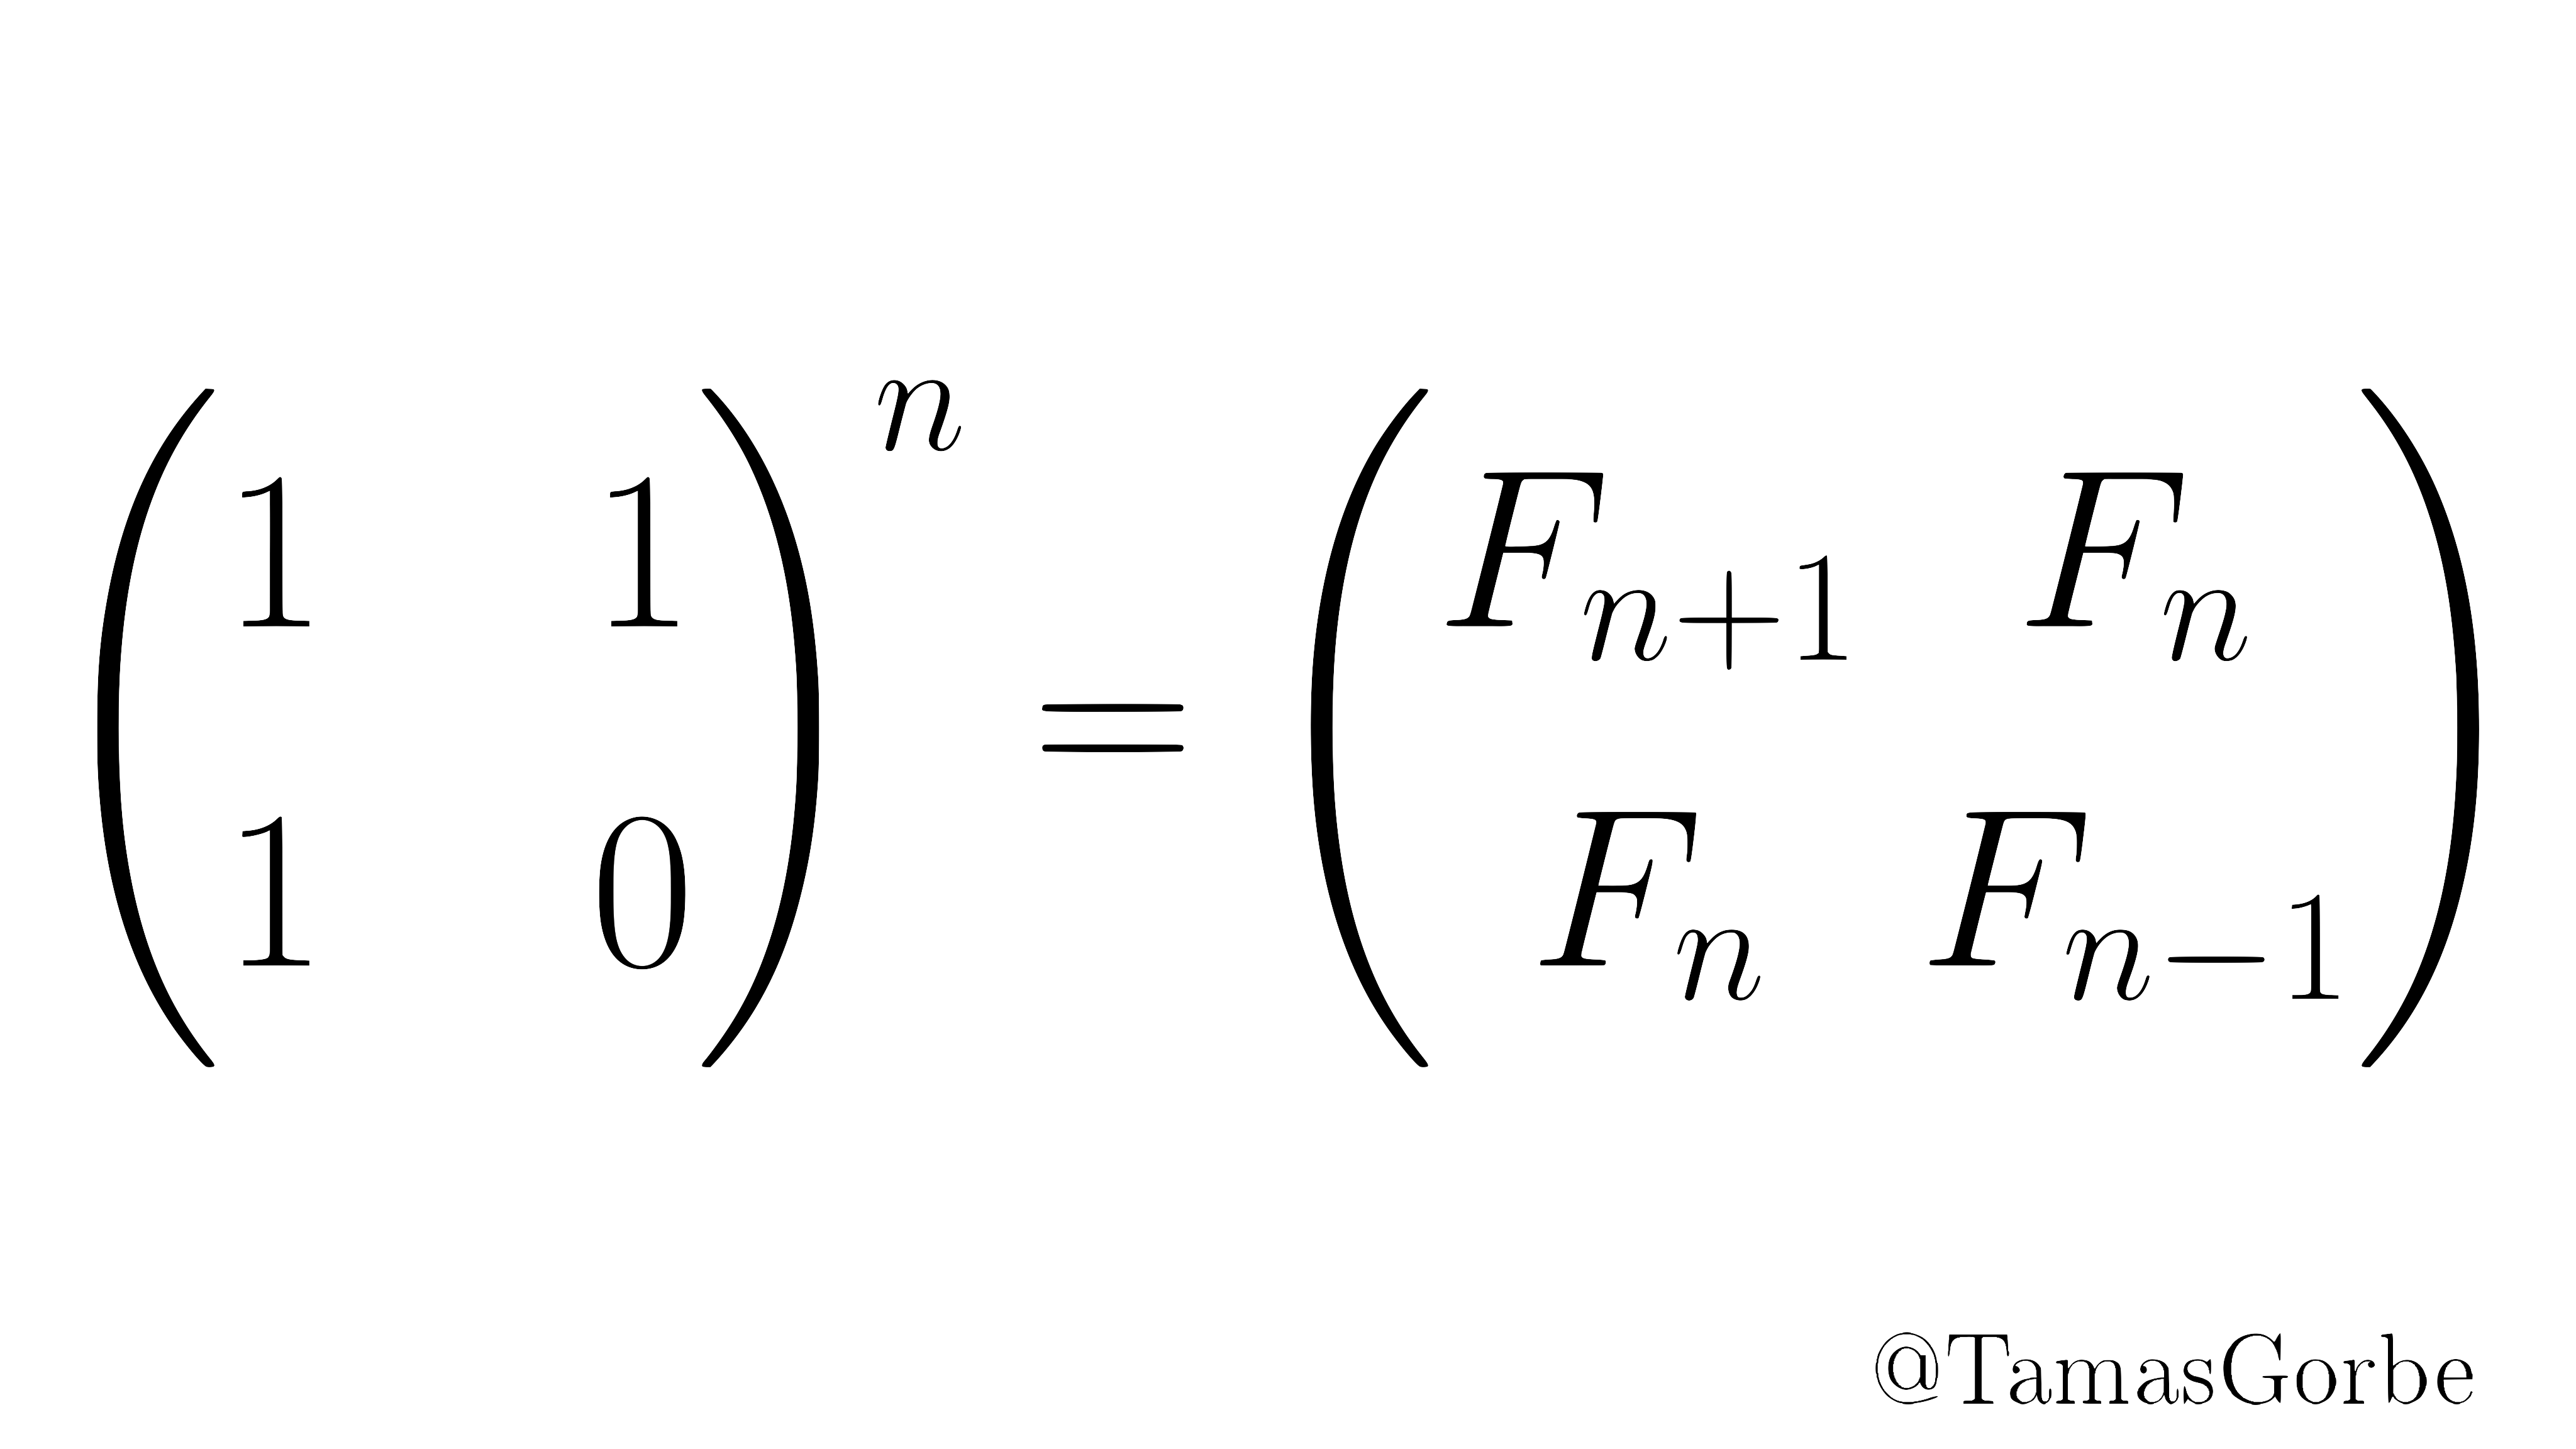
\includegraphics[width=1\textwidth]{imagenes/imagenes03/T03IM03.png}
\end{figure}

\end{myexampleblock}


\subsection{Cuestiones}

\begin{enumerate}[Q. 1] 

\item Sea $A_{m \times n}$

a) ¿Existe una matriz $B$ tal que $BA$ sea una matriz fila?, ¿cuál es su dimensión?

b) ¿Existe una matrz $B$ tal que $AB$ sea una matriz fila?, ¿cuál es su dimensión?

c) Si $AB$ es una matriz cuadrada, ¿qué dimensión tiene la matriz $B^TA^T$?

\rotatebox{180}{\leftline{\textcolor{gris}{\scriptsize{\hspace{5mm}  Ayuda: haz un análisis dimensional en cada caso. }}}}.

\item Considera las matrices $A_{m \times n}\; ; \; \; B_{p \times q}\;$. ¿Qué relación debe haber enre $m,n,p,q$ para que exista:?

a) $(AB)^{-1}$; \hspace{5mm} b) $A^2-B^2$; \hspace{5mm} c) $AB^T-A$

\rotatebox{180}{\leftline{\textcolor{gris}{\scriptsize{\hspace{5mm}  Ayuda: haz un análisis dimensional. }}}}.

\item Sean $A, B$ y $C$ tres matrices tales que $ABC$ es una matriz  $3 \times 2$ y $AC^T$ es una matriz cuadrada. Encuentra las dimensiones de $A$, $B$ y $C$.

\rotatebox{180}{\leftline{\textcolor{gris}{\scriptsize{\hspace{5mm}  Ayuda: haz un análisis dimensional. }}}}.

\item Si con las matrices $A,B,C$ y $D$ se pueden hacer las operaciones $(A+D)C^T; \; CBT; \text{ y }B^2$, ¿cuál de las operaciones siguientes se pede hacer:?

a) $\; CBD)^T\quad$ b) $\; C(D+A)B\quad$ c) $\; (BA^TD)^2\quad $ d) $\; (A^t+D^T)^2C$

\rotatebox{180}{\leftline{\textcolor{gris}{\scriptsize{\hspace{5mm}  Ayuda: solo el apartado c). }}}}.

\item  ?`Qué efecto tiene multiplicar una matriz diagonal de orden $3$, $\; D=Diag(\alpha,\beta,\gamma)=\left( \begin{array}{ccc} \alpha&0&0 \\0&\beta&0 \\ 0&0&\gamma \end{array} \right)\;$ por una matriz cuadrada $A$ cualquiera?

\rotatebox{180}{\leftline{\textcolor{gris}{\scriptsize{\hspace{5mm}  Ayuda: $AD=(\; \alpha c_1(A), \beta c_2(A), \gamma c_3(A) \;)\; \quad (DA)^T=(\; \alpha f_1(A), \beta f_2(A), \gamma f_3(A)\: ))$ }}}}.

\item Demuestra que si $A\in \mathcal M_{2 \times 2} \to (A^T)^2=(A^2)^T$

\rotatebox{180}{\leftline{\textcolor{gris}{\scriptsize{\hspace{5mm}  Ayuda: \scriptsize{$A=\left( \begin{matrix} a&b\\c&d \end{matrix} \right)$ y efectua las operaciones.} }}}}.

\item Encuentra las matrices $X$ que conmutan con $A=\left( \begin{matrix} 1&1\\1&1 \end{matrix} \right)$

\rotatebox{180}{\leftline{\textcolor{gris}{\scriptsize{\hspace{5mm}  Ayuda: $X=\left( \begin{matrix} a&b\\c&d \end{matrix} \right) \to AX=XA \Rightarrow X=\left( \begin{matrix} a&b\\b&a \end{matrix} \right)$ }}}}.

\item Encuentra las matrices $X$ que conmutan con $A=\left( \begin{matrix} 1&1\\0&1 \end{matrix} \right)$

\rotatebox{180}{\leftline{\textcolor{gris}{\scriptsize{\hspace{5mm}  Ayuda: $X=\left( \begin{matrix} a&b\\c&d \end{matrix} \right) \to AX=XA \Rightarrow X=\left( \begin{matrix} a&b\\0&a \end{matrix} \right)$ }}}}.

\item (*) Encuentra las matrices $X$ de segundo orden tales que $X^2=X$

\rotatebox{180}{\leftline{\textcolor{gris}{\scriptsize{\hspace{5mm}  Ayuda: $X:\; 
\left( \begin{matrix} 0&0\\0&0  \end{matrix} \right); \; 
\left( \begin{matrix} 1&0\\0&1  \end{matrix} \right); \; 
\left( \begin{matrix} a& \sqrt{a-a^2}\\ \sqrt{a-a^2}&1-a  \end{matrix} \right); \; 
 \left( \begin{matrix} a&\-sqrt{a-a^2}\\-\sqrt{a-a^2}&1-a  \end{matrix} \right) $ }}}}.

\item Demuestra que las matrices $M=\left( \begin{matrix} x&y\\y&x  \end{matrix}\right)$ e $N=\left( \begin{matrix} u&v\\v&u  \end{matrix}\right)$, conmutan.

\rotatebox{180}{\leftline{\textcolor{gris}{\scriptsize{\hspace{5mm}  Ayuda: $AB=BA$}}}}.

\item Prueba que $\forall A\in \mathcal M_{n \times n}$ se cumple que $A\cdot A^T$ es simetrica.

\rotatebox{180}{\leftline{\textcolor{gris}{\scriptsize{\hspace{5mm}  Ayuda: Calcula $(AA^T)^T$ y usa propiedades de la trasposición. (lema \ref{producto-traspuestas}) }}}}.

\item $M_{m \times n} \to MM^T \text { y } M^TM\; $ son, ambas, matrices simétricas.

\rotatebox{180}{\leftline{\textcolor{gris}{\scriptsize{\hspace{5mm}  Ayuda: $S$ simétrica si $S^T=T$ y usa propiedades de la trasposición. (lema \ref{producto-traspuestas}) }}}}.  

\item Prueba que si $A$ es idempotente, $A^2=A$, entonces, si  $B=2A-I$, se cumple que $B^2=I$

\rotatebox{180}{\leftline{\textcolor{gris}{\scriptsize{\hspace{5mm}  Ayuda: $B^2=B\cdot B=(2A-I)\cdot (2A-I)= \cdots$ }}}}.

\item (**) Encuentra todas las matrices ortogonales de orden 2, es decir, matrices $M$ tales que $MM^T=I \;\; (\;M^{-1}=M^T \;)$

\rotatebox{180}{\leftline{\textcolor{gris}{\scriptsize{\hspace{5mm}  Ayuda: $M=\left( \begin{matrix} a&b\\c&d   \end{matrix} \right) \to  
\left( \begin{matrix} \cos \theta & \sin \theta \\ -\sin \theta & \cos \theta   \end{matrix} \right) ; \; 
\left( \begin{matrix}  \cos \phi & \sin \phi \\ \sin \phi & - \cos \phi  \end{matrix} \right) ; \; \forall \theta,\phi \in \mathbb R$}}}}.

\item Sea $A$ una matriz cuadrada de orden $n$ tal que $A^2=0$:

a) Comprueba que $(A+I)^2=2A+I$

b) $B=I-A \; ; \quad C=A+I\;$. Comprueba que una es inversa de la otra.

\rotatebox{180}{\leftline{\textcolor{gris}{\scriptsize{\hspace{5mm}  Ayuda: a) $0$ es la matriz nula; $\quad$ b) calcula $BC$ }}}}.

\item Considera matrices triangulares cualquiera de orden 3 y comprueba que la suma, el producto por un número y el producto de matrices triangulares es triangular.

\rotatebox{180}{\leftline{\textcolor{gris}{\scriptsize{\hspace{5mm}  Ayuda: $A=\left( \begin{matrix} a&b&c\\0&d&e\\0&0&f  \end{matrix} \right); quad B=\left( \begin{matrix} x&y&z\\0&p&q\\0&0&r  \end{matrix} \right)  \to A+B; \; kA; \; AB$   }}}}.

\item Si la matriz $A$, de orden $n$, es invertible, entonces, la matriz $3A$:

\begin{multicols}{2}
\hspace{-11mm} \small{a) Es invertible y su inversa vale $3A^{-1}$}

\hspace{-11mm} \small{b) Es invertible y su inversa vale $3^n A^{-1}$}

\hspace{-6mm} \small{c) Es invertible y su inversa vale $\frac 1 3 A^{-1}$}

\hspace{-5mm}\small{d) No necesariamente es invertible.}
\end{multicols}

\rotatebox{180}{\leftline{\textcolor{gris}{\scriptsize{\hspace{5mm}  Ayuda: La respuesta correcta es la c) }}}}.

%\item

%\rotatebox{180}{\leftline{\textcolor{gris}{\scriptsize{\hspace{5mm}  Ayuda: }}}}.

%\item

%\rotatebox{180}{\leftline{\textcolor{gris}{\scriptsize{\hspace{5mm}  Ayuda: }}}}.

	
\end{enumerate}

\clearpage

\section{Resumen}

\begin{myalertblock}{Resumen de matrices}

$A=\left[
\begin{matrix}
a_{11} & a_{12} & \cdots & a_{1j} & \cdots & a_{1n} \\
a_{21} & a_{22} & \cdots & a_{2j} & \cdots & a_{2n} \\
a_{31} & a_{32} & \cdots & a_{3j} & \cdots & a_{3n} \\
\vdots & \vdots & \ddots & \vdots & \ddots & \vdots \\
a_{i1} & a_{i2} & \cdots & \boxed{a_{ij}} & \cdots & a_{in} \\
\vdots & \vdots & \ddots & \vdots & \ddots & \vdots \\
a_{m1} & a_{m2} & \cdots & a_{mj} & \cdots & a_{mn} \\
\end{matrix}
\right]$
\footnotesize{$= [a_{ij}]_{m \times n} \; \begin{cases}0\le i \le m; \\ 0\le j \le n\end{cases}$}

\vspace{3mm}
\centerline{$\boxed{\; \boldsymbol{A_{\;  (num. \; filas)\; \times \; (num. \; columnas) }}\; }$}

\vspace{2mm} Traspuesta: $\quad (a_{ij})^T=(a_{ji})$

\vspace{2mm} Producto por un número real: $\quad k(a_{ij})=(ka_{ij})$

\vspace{2mm} Suma: $\quad (a_{ij})_{m \times n}\; + \; (b_{ij})_{m \times n}=(a_{ij}+b_{ij})_{m \times n}$

\hspace{12mm} asociaiva, conmutativa, neutro $\boldsymbol{0}$, opuesto $-A$

\vspace{2mm} Producto: $\quad (a_{il})_{m \times \cancel{n}} \; \cdot \;(b_{lj})_{\cancel{n} \times p} \; = \; (f_i(A)\cdot c_j(B))_{m \times p}$

\hspace{15mm} \scriptsize{$AB \neq BA$, asociativa, distributivas, neutro $IA=AI=A$, inversa $A^{1}$}\footnotesize{.}

\hspace{12mm} $\quad A \in \mathcal M_n: \quad \exists A^{-1}\; / \; AA^{-1}=A^{-1}A=I$

\vspace{2mm} Potencias:  $\quad M\in \mathcal M_n :\quad M^n$

\vspace{2mm} Propiedades: $(A+B)^T=A^T+B^T \quad $ $(AB)^T=B^TA^T \quad $ $(AB)^{-1}=B^{-1}A^{-1} \quad $ $(A^{-1})^{-1}=A \quad $ $(A^T)^{-1}=(A^{-1})^T$

\vspace{2mm} Inversa por Gaus: $ \quad [\; A \; | \; I \; ] \; \to \text{ transf. Gauss } \to  \; [\; I \; | \; \boldsymbol{ A^{-1} } \; ] $\normalsize{.}

\end{myalertblock}


%$A=\left( \begin{matrix}   \end{matrix}\right)$

	%\begin{figure}[H]
		%\centering
		%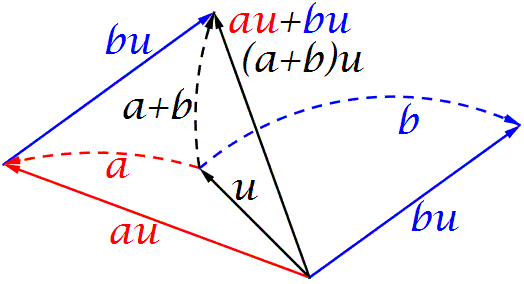
\includegraphics[width=0.5\textwidth]{imagenes/imagenes01/T01IM01.png}
		%\caption{Los dos problemas clásicos del cálculo: trazado de tangentes y áreas bajo curvas.}
	%\end{figure}
		
%varios párrafos encuadrados - explicaciones ad hoc
%\centering{
%\fbox{
%\parbox{0.95\textwidth}{
%varios
%
%$parrafos
%
%dentro
%}
%}
%}
% \justify


%\rotatebox{180}{\leftline{\textcolor{gris}{tararí}}}.